\documentclass[12pt,a4paper]{report}

% ================================================================
%  AIT Master's Thesis Format – January 2026
%  Forensically verified against Master_s_Thesis_Format_January_2026.docx
%
%  Verified specs:
%   Paper:       A4, all margins = 1.000 inch
%   Body font:   Times New Roman 12pt, justified, NO first-line indent
%   Line spacing: 1.5x  (Word line=360 auto ≡ \setstretch{1.5})
%   Chapter H1:  14pt Bold TNR, centred, "CHAPTER X  TITLE" on one line
%   Section H2:  12pt Bold TNR, left
%   Subsect H3:  12pt Bold Italic TNR, left
%   Fig caption: 12pt Bold TNR, centred, below figure, "Figure X.X. …"
%   Tbl caption: 12pt Normal TNR, centred, above table,  "Table X.X. …"
%   Tables:      APA 3-line style — top+midrule+bottomrule, NO verticals,
%                NO shading, all text TNR 12pt (header NOT bold)
%   References:  APA author-year style
% ================================================================

\usepackage{amsmath,amssymb}
\usepackage{graphicx}
\usepackage{float}
\usepackage{multirow}
\usepackage{booktabs}          % \toprule \midrule \bottomrule (APA tables)
\usepackage{enumitem}
\usepackage[T1]{fontenc}
\usepackage[utf8]{inputenc}
\usepackage{listings}
\usepackage{tcolorbox}
\usepackage{caption}
\usepackage{subcaption}

% ---- AIT: Times New Roman ----
\usepackage{mathptmx}

% ---- AIT: A4, 1 inch all margins ----
\usepackage[a4paper,
            top=1in, bottom=1in, left=1in, right=1in,
            headheight=14pt, headsep=0.2in, footskip=0.3in]{geometry}

% ---- AIT: 1.5x line spacing (Word line=360 lineRule=auto) ----
\usepackage{setspace}
\setstretch{1.5}

% ---- AIT: No paragraph indent, small skip between paragraphs ----
\setlength{\parindent}{0pt}
\setlength{\parskip}{4pt}

% ---- Colours ----
\usepackage[table]{xcolor}
\definecolor{nodeblue}{RGB}{52,120,190}
\definecolor{nodeorange}{RGB}{230,120,30}
\definecolor{nodegreen}{RGB}{60,160,80}
\definecolor{arrowgray}{RGB}{100,100,100}
\definecolor{boxblue}{RGB}{220,235,250}
\definecolor{boxorange}{RGB}{255,235,210}
\definecolor{boxgreen}{RGB}{210,245,220}
\definecolor{boxred}{RGB}{255,220,220}
\definecolor{boxgray}{RGB}{240,240,240}

% ---- TikZ ----
\usepackage{tikz}
\usepackage{pgfplots}
\pgfplotsset{compat=1.18}
\usetikzlibrary{shapes.geometric, arrows.meta, positioning, fit,
                backgrounds, calc, decorations.pathreplacing, shapes.multipart}

\usepackage{hyperref}
\hypersetup{colorlinks=false, hidelinks}

% ================================================================
%  AIT CAPTION FORMATTING (forensically verified)
%
%  Figure caption (Caption style in template):
%    - TNR 12pt BOLD, centred, BELOW figure
%    - "Figure X.X. Description" (dot after number)
%
%  Table title (TableTitle style in template):
%    - TNR 12pt NOT bold, centred, ABOVE table
%    - "Table X.X. Description" (dot after number)
%    - Double-spaced (line=480 in Word) — use \doublespacing in caption
% ================================================================

\captionsetup[figure]{
  font        = {normalsize, bf},
  labelfont   = {normalsize, bf},
  labelsep    = period,
  justification = centering,
  position    = below,
  skip        = 6pt
}
\captionsetup[table]{
  font        = normalsize,
  labelfont   = normalsize,
  labelsep    = period,
  justification = centering,
  position    = above,
  skip        = 4pt
}

% ================================================================
%  AIT HEADING FORMAT (verified from numbering XML)
%
%  Heading1: 14pt Bold TNR, centred — auto-prefix "CHAPTER X" 
%            then title on SAME LINE (Word autonumber = "CHAPTER %1")
%  Heading2: 12pt Bold TNR, left  — auto-prefix "X.X"
%  Heading3: 12pt Bold Italic TNR, left — auto-prefix "X.X.X"
% ================================================================
\usepackage{titlesec}

% Chapter: "CHAPTER X" on line 1, "TITLE" on line 2 — both centred 14pt bold
% Matches AIT template screenshot: two-line display format
\titleformat{\chapter}[display]
  {\normalfont\fontsize{14}{17}\bfseries\centering}
  {CHAPTER \thechapter}
  {0pt}
  {\MakeUppercase}
\titlespacing*{\chapter}{0pt}{0pt}{24pt}

% Section: "1.1  Title" — 12pt bold, left
\titleformat{\section}
  {\normalfont\fontsize{12}{14}\bfseries}
  {\thesection\quad}
  {0em}{}
\titlespacing*{\section}{0pt}{12pt}{4pt}

% Subsection: "1.1.1  Title" — 12pt bold italic, left
\titleformat{\subsection}
  {\normalfont\fontsize{12}{14}\bfseries\itshape}
  {\thesubsection\quad}
  {0em}{}
\titlespacing*{\subsection}{0pt}{10pt}{3pt}

% Subsubsection: "1.1.1.1  Title" — 12pt bold italic, left
\titleformat{\subsubsection}
  {\normalfont\fontsize{12}{14}\bfseries\itshape}
  {\thesubsubsection\quad}
  {0em}{}
\titlespacing*{\subsubsection}{0pt}{8pt}{2pt}

% ================================================================
%  Page numbers: bottom centre (AIT footer)
% ================================================================
\usepackage{fancyhdr}
\pagestyle{fancy}
\fancyhf{}
\renewcommand{\headrulewidth}{0pt}
\fancyfoot[C]{\thepage}
\fancypagestyle{plain}{%
  \fancyhf{}
  \renewcommand{\headrulewidth}{0pt}
  \fancyfoot[C]{\thepage}
}

% ================================================================
%  Code block (single-spaced inside tcolorbox)
% ================================================================
\lstset{breaklines=true, basicstyle=\footnotesize\ttfamily, lineskip=0.4ex}
\tcbuselibrary{listingsutf8}
\tcolorboxenvironment{lstlisting}{
  colback=gray!5!white, colframe=gray!80!black, boxrule=0.5pt, arc=3pt
}

% ================================================================
%  APA reference hanging indent helper
% ================================================================
\usepackage{natbib}
\setlength{\bibhang}{0.5in}
\setlength{\bibsep}{0pt}

% ================================================================
\begin{document}

    \pagenumbering{roman}
    \setcounter{page}{1}
\thispagestyle{empty}

\vspace*{\fill}

\begin{center}
        {\Large \bfseries Customer Journey Path Optimization}

    \vspace{9em}

    by
    \begin{center}
        Yosakorn Sirisoot \,| \, Aye Khin Khin Hpone  \\[0.5em]
    {\small   126512 \,|\, Yolanda Lim 125970 }
    \end{center}

\vfill

    \begin{center}AT70.02 -- Algorithms Design and Analysis\end{center}

    \vspace{3em}
    
    \begin{tabular}{l}
        Instructor: Dr.\ Chantri Polprasert \\
        Teaching Assistant: Puskar Adhikari
    \end{tabular}

    \vspace{9em}

    Asian Institute of Technology\\
    School of Engineering and Technology\\
    Thailand\\
    January 2026
\end{center}




\vspace*{\fill}

    \phantomsection
\addcontentsline{toc}{chapter}{\bf ABSTRACT}

\begin{center}
    \large{\bf ABSTRACT}
\end{center}

This project addresses the problem of identifying optimal conversion paths in large-scale customer journey graphs. User interaction sequences are modeled as a directed weighted graph $G=(V,E)$, where edge weights encode the negative log-probability of each state transition, enabling maximum-probability path search to be solved as a shortest-path problem using Dijkstra's algorithm.

Two algorithms are proposed and analyzed. The \textbf{Baseline Dijkstra} algorithm provides globally optimal solutions in $O(|E|\log|V|)$ time. The \textbf{Probability-Pruned Dijkstra} extends the baseline with a threshold parameter $\tau$ that discards low-probability partial paths during traversal, reducing the effective search space to $O(|E'|\log|V|)$ with $|E'|\leq|E|$ while converging to the baseline as $\tau\to 0$.

Both algorithms are evaluated on synthetic graphs up to 50,000 nodes across varying edge densities and probability distributions. The project provides formal correctness arguments, theoretical complexity analysis, and a fully specified empirical evaluation plan measuring runtime, peak memory usage, and solution quality. Results are expected to demonstrate a controllable efficiency--optimality trade-off, with the pruned algorithm achieving meaningful speedups at small optimality cost for moderate threshold values.


    \clearpage
    \phantomsection
    \renewcommand{\contentsname}{%
      \normalfont\fontsize{14}{17}\bfseries\MakeUppercase{Contents}}
    \tableofcontents

    \cleardoublepage
    \pagenumbering{arabic}

    \chapter{INTRODUCTION: PROBLEM DESCRIPTION AND MOTIVATION}

\section{Background of the Study}

Understanding how users navigate through digital systems---such as e-commerce websites, mobile applications, and customer support platforms---is essential for improving conversion rates, user satisfaction, customer retention, and operational efficiency. User interaction data captures detailed behavioural patterns that reflect how users interact with different system components. Customer journeys, represented as sequences of interaction states (e.g., \emph{Landing $\rightarrow$ Browse $\rightarrow$ Product $\rightarrow$ Cart $\rightarrow$ Checkout}), provide a structured framework for analyzing these behaviours.

Modern digital systems generate millions of user sessions and thousands of interaction states, forming large and complex navigation graphs across websites and online platforms. When aggregated, these journeys form large directed graphs with numerous states and transitions. The scale and complexity of such graphs make efficient computational analysis a necessity, motivating the use of algorithmic approaches grounded in graph theory and data mining.

\section{Statement of the Problem}

As the volume and complexity of user interaction data continue to grow, identifying meaningful and optimal customer journeys becomes increasingly challenging. From a business perspective, customer journey dynamics directly influence conversion rates, revenue generation, customer retention, and user satisfaction. Even small improvements in the probability of reaching a conversion state can result in significant financial gains at scale.

Na\"{i}ve analytical methods, such as exhaustive path enumeration or simple frequency-based techniques, do not scale. In large graphs, the number of possible simple paths increases combinatorially, rendering exhaustive enumeration computationally infeasible. Furthermore, directly multiplying many small transition probabilities along a path leads to numerical underflow---a form of arithmetic precision loss that makes na\"{i}ve probability computation unreliable for longer paths.

The key challenge is therefore to identify optimal customer journeys efficiently and numerically stably at scale. Core tasks include finding highest-probability conversion paths and analyzing scalability across large graphs, each posing distinct challenges in graph traversal, optimization, and algorithm design that require careful data structure selection.

\section{Objectives}

The objective of this study is to design and implement an efficient algorithmic framework for customer journey path optimization grounded in graph theory and classical algorithm design principles. Specifically, the project will model customer journey data as a directed weighted graph, where nodes represent interaction states and edges represent transition probabilities between states.

The primary focus is to compute optimal conversion paths under probabilistic constraints. To achieve this, transition probabilities will be transformed into additive non-negative edge weights using the negative logarithm, enabling the application of Dijkstra's shortest-path algorithm for maximum-probability path computation. This transformation also addresses the numerical underflow problem by converting multiplicative probability products into additive sums. The project will implement Dijkstra's algorithm as a baseline approach and further propose an optimized probability-pruned search strategy that reduces the exploration of low-probability paths to improve computational efficiency.

In addition to correctness, the project aims to formally analyze the theoretical time and space complexity of both the baseline and optimized algorithms. Empirical performance evaluations will be conducted on graphs of varying sizes and densities to examine scalability, runtime behaviour, and trade-offs between computational efficiency and path optimality. Through these analyses, the project seeks to demonstrate how careful algorithm design and data structure selection influence performance in large-scale navigation graphs.

\noindent\textbf{Original contribution.} This study contributes a threshold-based pruning strategy integrated with Dijkstra's algorithm for probabilistic navigation graphs, evaluated through empirical complexity analysis and an explicit time--optimality trade-off characterization. Unlike heuristic approaches (A*) that require a problem-specific admissible heuristic, or rank-based methods (beam search) that provide no convergence guarantee, the proposed pruning is deterministic, requires no domain-specific heuristic, and formally converges to the globally optimal solution as $\tau \to 0$.

A further objective is to identify the \emph{critical pruning threshold} $\tau_c$, defined as the value or narrow range of $\tau$ for which runtime improvement is maximized without causing a significant degradation in path quality. In this study, significance will be assessed empirically using the relative optimality gap $\Delta$ together with runtime speedup across all experimental configurations.

\section{Target Users}

The primary target users of this system include data analysts, product managers, and system designers working on digital platforms such as e-commerce websites, mobile applications, and customer support systems. The project is also intended for researchers and students interested in applying algorithm design and data structure concepts to real-world optimization problems. Insights derived from this work can support data-driven decision-making and contribute to improved system performance and user experience.

    \chapter{RELATED WORK AND BACKGROUND}

\section{Shortest-Path Algorithms for Conversion Path Optimization}

Dijkstra~\citep{dijkstra1959} introduced one of the most fundamental shortest-path algorithms for weighted graphs with non-negative edge weights. The algorithm incrementally explores nodes in order of increasing accumulated cost using a priority queue, guaranteeing optimality when all edge weights are non-negative. When implemented with a binary min-heap, it achieves a time complexity of $O(|E|\log|V|)$~\citep{cormen2009}. A theoretically superior bound of $O(|E| + |V|\log|V|)$ is achievable using Fibonacci heaps~\citep{fredman1987fibonacci}, though the practical overhead of Fibonacci heaps often makes binary-heap implementations preferable for moderately sized graphs. In the context of this project, Dijkstra's algorithm serves as the baseline, applied to a log-transformed probability graph where edge weights represent the negative log-probability of transitions. Its well-understood complexity and correctness guarantees make it the natural choice for baseline comparison and scalability analysis.

\section{Heuristic and Approximate Shortest-Path Approaches}

While Dijkstra's algorithm guarantees optimality, it explores the full reachable graph from the source. Informed search algorithms such as A*~\citep{hart1968astar} reduce exploration by using an admissible heuristic function to guide node expansion toward the target, achieving sub-Dijkstra runtime when a valid heuristic exists. Pearl~\citep{pearl1984heuristics} provides a comprehensive theoretical treatment of heuristic search, establishing formal conditions under which informed search algorithms guarantee optimal solutions. In probabilistic graph settings, however, designing a tight and admissible heuristic over log-probability weights is non-trivial, making heuristic approaches difficult to apply directly. Beam search offers an alternative approximation strategy by limiting the frontier to the top-$k$ most promising candidates at each step~\citep{cormen2009}. Although beam search can be very fast in practice, it provides no optimality guarantee and may miss the globally optimal path entirely. This project adopts a different approximation strategy---probability-threshold pruning---which is deterministic, parameter-controlled, and guarantees convergence to the optimal solution as the threshold approaches zero, offering a more principled trade-off than beam search. Unlike A*, which requires a problem-specific admissible heuristic that is difficult to define over log-probability edge weights, and unlike beam search, which discards nodes based on rank with no convergence guarantee, the proposed pruning operates directly on accumulated path cost against a single interpretable parameter $\tau$, requiring no domain-specific heuristic design and providing a formal convergence proof as $\tau \to 0$.

Another important family of shortest-path speedup methods is \emph{Contraction Hierarchies}, which accelerates queries by preprocessing the graph and adding shortcut edges to preserve shortest-path distances. Such methods are highly effective for static road-network-style graphs, but they are less naturally suited to the probabilistic customer-journey setting considered here, where transition weights are derived from behavioral data and experimental emphasis is placed on controllable approximation rather than heavy preprocessing. Nevertheless, Contraction Hierarchies provide an important point of comparison within the broader landscape of shortest-path acceleration methods.

\section{Markov Chain Models for Probabilistic Navigation}

The probabilistic transition model used in this project---where each user state transitions to the next with a fixed probability---is formally equivalent to a first-order Markov chain~\citep{norris1998markov}. Markov chains have been widely used to model sequential user behaviour in web navigation, recommendation systems, and clickstream analysis~\citep{rabiner1989hmm,baum1966statistical}. The maximum-probability path problem on a Markov chain is structurally identical to the Viterbi algorithm~\citep{viterbi1967error}, which finds the most likely state sequence in a Hidden Markov Model using dynamic programming in $O(|V|^2 T)$ time for $T$ time steps. However, the Viterbi algorithm is designed for sequences of fixed length, whereas the present problem involves finding the most probable \emph{path} from $s$ to $t$ in a general directed graph without a fixed path length. The log-probability shortest-path formulation adopted here generalizes the Viterbi principle to arbitrary directed graphs and applies it efficiently using Dijkstra's algorithm, which has better practical complexity on sparse graphs.

\section{Algorithmic Foundations of Efficient Graph Traversal}

Cormen et al.~\citep{cormen2009} provided a comprehensive treatment of graph algorithms, including shortest-path search, graph traversal, and priority-queue-based optimization techniques. The textbook formally analyzes time and space complexity, establishes correctness proofs for Dijkstra's algorithm, and discusses data structure choices including binary heaps and adjacency lists. These foundations directly support the design decisions in this project: the use of adjacency lists for $O(|V|+|E|)$ space, binary heaps for $O(\log|V|)$ extract-min and insert operations, and hash maps for $O(1)$ distance lookup. The log-probability weight transformation exploits the monotone relationship between probability maximization and shortest-path minimization, a standard technique in probabilistic graph optimization~\citep{manning2008nlp}.

\section{Sequential Pattern Mining for Frequent Journey Discovery}

Pei et al.~\citep{pei2001prefixspan} proposed PrefixSpan, a pattern-growth-based algorithm for mining frequent sequential patterns without candidate generation. By projecting the database based on frequent prefixes, PrefixSpan significantly reduces search space compared to Apriori-based approaches and demonstrated strong scalability on large sequence datasets. In the context of this project, PrefixSpan is conceptually relevant as a method for identifying frequently taken customer journey paths without enumerating all possible sequences. Its prefix-based pruning principle shares conceptual similarities with the threshold-based pruning strategy proposed in this work, where low-probability path prefixes are discarded early to reduce the effective search space.

\section{Survey of Frequent and Sequential Pattern Mining Techniques}

Han et al.~\citep{han2007sequential} presented a comprehensive survey of frequent pattern mining methods, covering association rules, sequential patterns, and constrained pattern mining. The survey highlights key challenges including scalability, pattern explosion, and the need for efficient pruning strategies. These challenges closely mirror those encountered in customer journey analysis, where the number of simple paths from source to target grows combinatorially with graph size. This project draws on the general principle of threshold-based pruning to control computational complexity, filtering out low-probability paths before full expansion in a manner analogous to minimum support thresholds in frequent pattern mining.

\section{Modeling User Navigation as Directed Graphs}

Bucklin and Sismeiro~\citep{bucklin2003clickstream} modeled user browsing behaviour using clickstream data, representing navigation patterns as structured sequences and probabilistic transition graphs. Their empirical analysis demonstrated that user navigation can be effectively captured using probabilistic transition models, providing insights into user behaviour and engagement at scale. Liu~\citep{liu2011webmining} further surveyed web usage mining techniques---including clickstream analysis, hyperlink analysis, and content mining---providing a broader context for how navigation data is processed into actionable graph representations. This work directly supports the modeling approach adopted in this project, where customer journeys are represented as directed weighted graphs derived from interaction sequences, and transition probabilities are estimated from session frequency counts using maximum likelihood estimation.

\section{Probabilistic Models for Navigation and Path Selection}

Resnick and Varian~\citep{resnick1997recommender} discussed probabilistic models of user behaviour, including transition-based navigation models that capture the likelihoods of moving between system states. Such models are commonly used to estimate user preferences and navigation patterns in large-scale recommendation and information retrieval systems. The probabilistic transition modeling approach adopted in this project---assigning edge weights as negative log-probabilities and finding the minimum-weight path---is consistent with the broader class of log-linear models used in language modeling and information retrieval~\citep{manning2008nlp,manning2008ir}, where the negative log-likelihood serves as a natural additive cost function.

\section{Scalable Graph Processing and Large-Scale Navigation Analysis}

Recent advances in large-scale graph processing systems further emphasize the importance of efficient algorithmic design when analyzing massive navigation graphs. Malewicz et al.~\citep{malewicz2010pregel} introduced Pregel, a vertex-centric computational model for scalable graph processing, demonstrating how distributed systems can efficiently handle graphs containing millions or billions of edges. Subsequent research in large-scale graph analytics has examined optimization strategies for traversal, pruning, and distributed processing to reduce computational overhead in dense and evolving networks~\citep{sahu2020scaling}. These studies reinforce the practical relevance of designing efficient path-search algorithms and pruning strategies when working with large customer journey graphs, where computational complexity grows rapidly with graph size. The present project builds upon these principles by evaluating algorithmic efficiency and search-space reduction techniques within a single-machine, controlled experimental framework, where the goal is to characterize complexity empirically rather than to achieve distributed scalability.

\vspace{0.5cm}

\noindent The reviewed literature establishes a strong theoretical and methodological foundation for this project. Dijkstra's algorithm~\citep{dijkstra1959} and its complexity analysis~\citep{cormen2009,fredman1987fibonacci} provide the basis for the baseline implementation and complexity comparison. The Markov chain and Viterbi frameworks~\citep{norris1998markov,viterbi1967error,rabiner1989hmm} situate the probabilistic path problem in a well-studied theoretical context. Heuristic search methods~\citep{hart1968astar,pearl1984heuristics} and approximate approaches establish the landscape of alternatives against which the pruning strategy is positioned. Sequential pattern mining techniques~\citep{pei2001prefixspan,han2007sequential} and clickstream modeling~\citep{bucklin2003clickstream,liu2011webmining} validate the representation and motivate pruning as a scalability mechanism. Probabilistic modeling literature~\citep{resnick1997recommender,manning2008nlp} supports the log-probability transformation. Scalable graph systems~\citep{malewicz2010pregel,sahu2020scaling} contextualize the scalability challenges addressed. The Erd\H{o}s--R\'{e}nyi model~\citep{erdosrenyi1960} grounds the synthetic data generation methodology, and real-world benchmarks~\citep{retailrocket2015,uci2008eshop} validate experimental generalizability.

\section{Graph Cycles in Customer Journey Navigation}

A critical modeling question is whether the customer journey graph contains cycles---that is, whether a user may return to a previously visited state, such as \textit{Landing $\to$ Browse $\to$ Product $\to$ Browse}. Real-world clickstream data frequently exhibits such revisitation behaviour~\citep{bucklin2003clickstream}: users loop between states (e.g., browsing multiple product pages before adding to cart) before eventually converting or abandoning the session. The customer journey graph is therefore modeled as a general directed weighted graph that \emph{may contain cycles}.

A key concern is whether Dijkstra's algorithm remains correct on cyclic graphs. Cormen et al.~\citep{cormen2009} establish that Dijkstra's algorithm is correct on any directed graph with non-negative edge weights, regardless of whether cycles are present. The log-probability transformation $w(u,v) = -\log\,p(u,v) \geq 0$ guarantees non-negativity for all $p(u,v) \in (0,1]$, so Dijkstra's algorithm is directly applicable to cyclic navigation graphs without any cycle-detection preprocessing. Since each cycle traversal adds strictly positive cost, the algorithm naturally avoids cycling: once a node is finalized, it is never re-extracted from the priority queue. This property means no modifications to the standard algorithm are required to handle the cyclic structure that is inherent in real user navigation data.

\section{Synthetic Graph Generation for Controlled Evaluation}

To evaluate algorithmic performance in a controlled and reproducible manner, synthetic graphs are used as the primary experimental dataset. The generation methodology is grounded in the Erd\H{o}s--R\'{e}nyi random graph model~\citep{erdosrenyi1960}, which provides a theoretically principled basis for generating random directed graphs with predictable structural properties (connectivity, degree distribution) at a given size and density.

Graphs are generated as follows. Each node represents an interaction state. For each graph instance with $|V|$ nodes and target average out-degree $\bar{d} \in \{2, 5, 10\}$, directed edges are sampled independently such that the expected number of edges is $\bar{d} \cdot |V|$. Transition probabilities are assigned under two distributions: (i) \textbf{uniform} $\mathcal{U}(0.1, 1.0]$, simulating balanced navigation, and (ii) \textbf{skewed power-law} with exponent $\alpha = 2$, where a small number of transitions carry high probability and the majority carry low probability, reflecting the heterogeneous click patterns observed in real e-commerce data~\citep{bucklin2003clickstream,retailrocket2015}. For each node, outgoing probabilities are normalized to $\sum_v p(u,v) \leq 1$, ensuring a valid sub-stochastic transition system. A fixed source $s$ and target $t$ are assigned per instance, with at least one valid $s$-to-$t$ path guaranteed by a depth-first seeding step. All experiments use fixed random seeds for full reproducibility.

Synthetic generation is preferred as the primary substrate because it allows independent control of $|V|$, $|E|$, and the probability distribution---three variables that cannot be decoupled in observational data. Real-world datasets (RetailRocket~\citep{retailrocket2015}, UCI E-Commerce Clickstream~\citep{uci2008eshop}) are used as secondary validation to confirm findings generalize beyond synthetic graphs.

\vspace{0.5cm}
\noindent\textbf{Research Gap.} Despite the extensive literature above, existing studies largely treat shortest-path computation~\citep{dijkstra1959,cormen2009}, probabilistic modeling~\citep{norris1998markov}, and sequential pattern mining~\citep{pei2001prefixspan} as separate problems. Limited work integrates all three within a unified framework tailored to customer conversion path analysis, with explicit treatment of cyclic navigation graphs, principled synthetic data generation~\citep{erdosrenyi1960}, and empirical characterization of the time--optimality trade-off of threshold-based pruning.

The present project addresses this gap by combining probabilistic transition modeling, threshold-controlled pruning, and Dijkstra's algorithm into a cohesive experimental framework. By systematically evaluating performance across diverse synthetic and real-world graph configurations---including cyclic graphs---the study bridges classical graph algorithms, Markov chain theory, and practical navigation graph analysis within a single experimental design. This work contributes a threshold-based pruning strategy integrated with Dijkstra's algorithm for probabilistic navigation graphs, evaluated through empirical complexity analysis and an explicit time--optimality trade-off characterization.

    \chapter{PROPOSED ALGORITHM AND DATA STRUCTURES}

\section{System Overview}

The \textit{Customer Journey Path Optimization} system will model user interactions as a directed weighted graph $G = (V, E)$, where each node $v \in V$ represents a discrete interaction state (e.g., \textit{Landing Page}, \textit{Search}, \textit{Product Page}, \textit{Cart}, \textit{Checkout}), and each directed edge $(u,v) \in E$ represents a user transition between states annotated with a transition probability $p(u,v) \in (0,1]$. The primary goal is to identify the most probable path from a designated source node $s$ to a target conversion node $t$.

Figure~\ref{fig:system_workflow} presents the end-to-end workflow process. The workflow process is organized into five sequential components: (1) data generation and preprocessing, (2) graph construction, (3) baseline path optimization using Dijkstra's algorithm, (4) optimized path search using probability-pruned Dijkstra, and (5) experimental evaluation and comparative analysis.

Two algorithms are proposed and compared throughout this chapter:
\begin{itemize}
    \item \textbf{Algorithm 1 --- Baseline Dijkstra on Log-Weights:} Standard Dijkstra's algorithm applied to the log-probability-transformed graph. Guarantees globally optimal paths in $O(|E|\log|V|)$ time.
    \item \textbf{Algorithm 2 --- Probability-Pruned Dijkstra:} Extension of Algorithm~1 with a pruning threshold $\tau$ that discards partial paths whose cumulative probability falls below $\tau$. Reduces expected runtime to $O(|E'|\log|V|)$, $|E'| \leq |E|$, with convergence to Algorithm~1 as $\tau \to 0$.
\end{itemize}

% ----------------------------------------------------------------
% FIGURE 1: System Workflow
% ----------------------------------------------------------------
\begin{figure}[h!]
\centering
\begin{tikzpicture}[
    node distance=0.6cm and 0.3cm,
    box/.style={rectangle, rounded corners=4pt, minimum width=2.6cm, minimum height=0.9cm,
                text centered, font=\small\bfseries, draw=black, thick},
    arrow/.style={-{Stealth[length=5pt]}, thick, color=arrowgray},
    label/.style={font=\scriptsize\itshape, text=gray}
]

% Step boxes
\node[box, fill=boxblue]  (s1) {Data Gen.};
\node[box, fill=boxblue, right=of s1]  (s2) {Graph Build};
\node[box, fill=boxorange, right=of s2] (s3) {Baseline Dijkstra};
\node[box, fill=boxgreen,  right=of s3] (s4) {Pruned Dijkstra};
\node[box, fill=boxgray,   right=of s4] (s5) {Evaluation};

% Arrows
\draw[arrow] (s1) -- (s2);
\draw[arrow] (s2) -- (s3);
\draw[arrow] (s3) -- (s4);
\draw[arrow] (s4) -- (s5);

% Sub-labels
\node[label, below=0.15cm of s1] {Synthetic \& Real};
\node[label, below=0.15cm of s2] {$G=(V,E),\; w(u,v)$};
\node[label, below=0.15cm of s3] {$O(|E|\log|V|)$};
\node[label, below=0.15cm of s4] {Threshold $\tau$};
\node[label, below=0.15cm of s5] {Metrics \& Trade-offs};

% Group bracket
\draw[decorate, decoration={brace, amplitude=6pt, mirror}, thick, color=nodeblue]
    ([xshift=-2pt, yshift=-1.1cm]s1.south west) -- ([xshift=2pt, yshift=-1.1cm]s5.south east)
    node[midway, below=8pt, font=\small\bfseries, color=nodeblue]
    {Customer Journey Path Optimization Workflow Process};
\end{tikzpicture}
\caption[System workflow overview]{Five-stage workflow process: data generation, graph construction, baseline Dijkstra, pruned Dijkstra, and experimental evaluation.}
\label{fig:system_workflow}
\end{figure}

\section{Problem Formulation}

\subsection{Graph Model and Inputs}

Customer interactions will be modeled as a directed graph $G = (V, E)$ with the following inputs:
\begin{itemize}
    \item $V$: the set of interaction states (nodes).
    \item $E \subseteq V \times V$: the set of directed transitions (edges).
    \item A transition probability function $p(u,v) \in (0,1]$ assigned to each edge $(u,v) \in E$.
    \item A designated source node $s \in V$ (e.g., Landing Page) and target node $t \in V$ (e.g., Checkout).
    \item A pruning threshold $\tau \in (0,1]$ used by the optimized algorithm to discard low-probability partial paths.
\end{itemize}

Figure~\ref{fig:journey_graph} illustrates a representative small customer journey graph to clarify the graph model.

% ----------------------------------------------------------------
% FIGURE 2: Example Customer Journey Graph
% ----------------------------------------------------------------
\begin{figure}[h!]
\centering
\begin{tikzpicture}[
    state/.style={circle, draw=black, thick, minimum size=1.15cm,
                  font=\small\bfseries, fill=boxblue},
    conv/.style={circle, draw=nodegreen!80!black, very thick, minimum size=1.15cm,
                 font=\small\bfseries, fill=boxgreen},
    src/.style={circle, draw=nodeorange!80!black, very thick, minimum size=1.15cm,
                font=\small\bfseries, fill=boxorange},
    epath/.style={-{Stealth[length=6pt]}, very thick, color=nodeblue},
    earrow/.style={-{Stealth[length=5pt]}, thick, color=black!40, dashed},
    elabel/.style={font=\scriptsize\itshape, fill=white, inner sep=1pt}
]
% ── Graph nodes (manual positioning for clarity) ──
\node[src]   (LP) at (0,0)     {LP};
\node[state] (SR) at (3.2,0)   {SR};
\node[state] (PP) at (6.4,1.4) {PP};
\node[state] (CT) at (6.4,-1.4){CT};
\node[conv]  (CK) at (9.6,1.4) {CK};

% ── Optimal path (solid blue) ──
\draw[epath] (LP) -- node[elabel,above]{$p=0.7$} (SR);
\draw[epath] (SR) -- node[elabel,above left]{$p=0.6$} (PP);
\draw[epath] (PP) -- node[elabel,above]{$p=0.8$} (CK);

% ── Alternative transitions (dashed) ──
\draw[earrow] (SR) -- node[elabel,below left]{$p=0.4$} (CT);
\draw[earrow] (CT) to[bend right=18] node[elabel,below right]{$p=0.3$} (CK);
\draw[earrow] (LP) to[bend right=30] node[elabel,below]{$p=0.3$} (CT);
\draw[earrow] (PP) -- node[elabel,right]{$p=0.2$} (CT);

% ── Legend box BELOW the graph, separated by white space ──
\node[draw=black!30, rounded corners=4pt, fill=white, inner sep=6pt,
      below=1.6cm of SR, xshift=1.8cm] (legbox) {%
  \begin{tabular}{@{}ll@{}}
    \tikz[baseline=-0.5ex]\draw[epath,shorten >=1pt] (0,0)--(0.55,0); &
      Optimal path $(s \!\to\! t)$\\[3pt]
    \tikz[baseline=-0.5ex]\draw[earrow,shorten >=1pt] (0,0)--(0.55,0); &
      Alternative transitions\\[3pt]
    \tikz[baseline=-0.5ex]\node[src,minimum size=0.38cm,inner sep=0pt,font=\tiny]{}; &
      Source $s$\ (LP = Landing Page)\\[3pt]
    \tikz[baseline=-0.5ex]\node[conv,minimum size=0.38cm,inner sep=0pt,font=\tiny]{}; &
      Target $t$\ (CK = Checkout)
  \end{tabular}
};
\end{tikzpicture}
\caption[Example customer journey graph]{Representative customer journey graph. Nodes are interaction states; LP = source $s$, CK = target $t$. Solid blue path LP$\to$SR$\to$PP$\to$CK is optimal ($\Pi^*=0.336$, log-cost$\approx1.091$); dashed edges are alternatives.}
\label{fig:journey_graph}
\end{figure}

\subsection{Probabilistic Path Objective and Outputs}

The graph in Figure~\ref{fig:journey_graph} shows five nodes connected by directed edges with transition probabilities. The optimal path LP$\to$SR$\to$PP$\to$CK (solid blue) achieves probability $0.7\times0.6\times0.8=0.336$. In log-space the edge weights are $-\log(0.7)\approx0.357$, $-\log(0.6)\approx0.511$, and $-\log(0.8)\approx0.223$, giving a total cost of approximately $1.091$ that Dijkstra's algorithm minimizes. Alternative lower-probability paths (dashed) are explored but not selected. Real graphs in this project will contain up to 50,000 nodes with sparse connectivity~\citep{bucklin2003clickstream}.

The goal is to find a path $P^* = (v_0 = s,\, v_1,\, \ldots,\, v_k = t)$ that maximizes the joint path probability~\citep{norris1998markov}:

\[
\max_{P} \prod_{(u,v) \in P} p(u,v)
\]

Directly multiplying many small probabilities causes numerical underflow~\citep{manning2008nlp}, a precision loss that renders long-path probability computations unreliable in floating-point arithmetic. To address this, each transition probability is transformed into an additive non-negative edge weight using the negative logarithm, a standard technique in probabilistic sequence modeling~\citep{viterbi1967error,rabiner1989hmm}:

\[
w(u,v) = -\log\bigl(p(u,v)\bigr)
\]

Since $p(u,v) \in (0,1]$, it follows that $w(u,v) \geq 0$ for all edges, satisfying the non-negativity requirement of Dijkstra's algorithm~\citep{cormen2009}. The maximization objective is then equivalently reformulated as a shortest-path minimization:

\[
\max \prod_{(u,v)\in P^*} p(u,v) \;\iff\; \min \sum_{(u,v)\in P^*} -\log\, p(u,v)
\]

If $p(u,v) = 0$ for any edge, that edge will be treated as infinite cost (non-traversable). If no path from $s$ to $t$ exists, the algorithm will report this correctly.

The system is expected to produce the following outputs:
\begin{itemize}
    \item The optimal or near-optimal path $P^* = (v_0 = s, v_1, \ldots, v_k = t)$.
    \item The path probability $\Pi^* = \prod_{(u,v)\in P^*} p(u,v)$.
    \item The log-transformed path cost $C^* = \sum_{(u,v)\in P^*} -\log\, p(u,v)$.
    \item Runtime and exploration metrics: execution time, peak memory usage, nodes explored, edges relaxed, and maximum priority queue size.
    \item Comparative performance results between the baseline and optimized algorithms across varying input sizes and threshold values.
\end{itemize}

\subsection{Constraints and Assumptions}

The following constraints and assumptions will govern the implementation:
\begin{itemize}
    \item Graph size may reach up to 50,000 nodes (hardware permitting).
    \item Graphs are assumed to be sparse ($|E| = O(|V|)$); an adjacency list will be used to maintain $O(|V|+|E|)$ space complexity~\citep{cormen2009}.
    \item Worst-case time complexity must remain polynomial.
    \item All transition probabilities are strictly positive; zero-probability edges are treated as non-traversable.
    \item A correct solution requires the baseline to return the globally optimal path, and the optimized algorithm to converge to the baseline when $\tau \to 0$.
\end{itemize}

\item The customer journey graph is allowed to contain directed cycles, reflecting realistic revisitation behavior (e.g., Browse $\rightarrow$ Product $\rightarrow$ Browse). No acyclicity assumption is imposed; correctness is preserved because the transformed edge weights remain non-negative, allowing Dijkstra's algorithm to operate correctly on cyclic graphs.

\section{Data Generation and Preprocessing}

\subsection{Synthetic Data Generation}

Synthetic customer journey graphs will serve as the primary dataset, providing full control over graph structure and enabling repeatable, scalable benchmarking. The generation methodology is grounded in the Erd\H{o}s--R\'{e}nyi random graph model~\citep{erdosrenyi1960}, which provides a theoretically principled basis for generating random directed graphs with predictable structural properties (connectivity and degree distribution) at a given size and density.

Graphs will be generated using the following procedure:

\begin{enumerate}
    \item Create $|V|$ nodes representing interaction states (e.g., Landing Page, Browse, Product Page, Cart, Checkout).
    \item For each node pair $(u,v)$, include a directed edge independently with probability $p_{\text{edge}} = \bar{d}/(|V|-1)$, where $\bar{d} \in \{2, 5, 10\}$ is the target average out-degree. This yields an expected total of $\bar{d} \cdot |V|$ edges, producing sparse graphs of varying density.
    \item Assign transition probabilities $p(u,v)$ to each edge under one of two distributions: (i) \textbf{uniform} $\mathcal{U}(0.1, 1.0]$, simulating balanced navigation behaviour; or (ii) \textbf{skewed power-law} with exponent $\alpha = 2$, where a small number of transitions carry high probability and the majority carry low probability, reflecting heterogeneous click patterns observed in real e-commerce data~\citep{bucklin2003clickstream}.
    \item Normalize outgoing probabilities for each node so that $\sum_v p(u,v) \leq 1$, ensuring a valid sub-stochastic transition system.
    \item Fix a designated source $s$ and target $t$, and guarantee at least one valid $s$-to-$t$ path using a depth-first path seeding step.
    \item Fix a random seed per configuration for full reproducibility across all 10 repeated runs.
\end{enumerate}

\noindent\textbf{Graph cycles.} Real customer journey data contains cycles: users frequently revisit states (e.g., \textit{Browse $\to$ Product $\to$ Browse $\to$ Cart}). The synthetic generator does \emph{not} enforce acyclicity; cycles arise naturally from the random edge-sampling procedure, mirroring real navigation behaviour. As established in Chapter~2, Dijkstra's algorithm remains fully correct on these cyclic graphs because the log-probability transformation $w(u,v) = -\log\,p(u,v) \geq 0$ guarantees non-negative edge weights~\citep{cormen2009}. Each cycle traversal adds strictly positive cost, so no node is ever re-finalized. No cycle detection or DAG preprocessing is required.

Synthetic generation is preferred as the primary substrate because it enables independent control of $|V|$, $|E|$, and the probability distribution---variables that cannot be decoupled in observational data. Input sizes will span three scales: small ($|V| \approx 1{,}000$), medium ($|V| \in [5{,}000,\; 10{,}000]$), and large ($|V|$ up to 50,000 nodes). Real-world datasets (RetailRocket~\citep{retailrocket2015}, UCI E-Commerce Clickstream~\citep{uci2008eshop}) are used as secondary validation benchmarks.

In addition to the Erd\H{o}s--R\'enyi-style sparse random generator, a second \emph{layered/stage-based graph generator} will be included to better reflect realistic customer-journey structure. In this generator, nodes are partitioned into ordered behavioral stages such as Awareness, Consideration, Intent, and Conversion, and transitions are sampled primarily between adjacent or near-adjacent stages, with limited backward or within-stage links to preserve realistic revisitation behavior. This provides a more domain-representative graph topology while retaining controlled variation in size, density, and probability distribution.

Using both generators strengthens the evaluation design: the random generator tests algorithmic behavior on generic sparse graphs, while the layered generator evaluates performance on more realistic customer-journey graphs.

\subsection{Real-World Clickstream Data}

Two real-world clickstream datasets will be used for secondary validation:

\begin{itemize}
    \item \textbf{RetailRocket E-Commerce Dataset}~\citep{retailrocket2015}: A publicly available Kaggle dataset containing approximately 2.7 million clickstream events across 235,000 items, collected from a real e-commerce platform. Sessions are extracted and state-transition sequences constructed from \texttt{view}, \texttt{addtocart}, and \texttt{transaction} events.
    \item \textbf{UCI E-Commerce Clickstream Dataset}~\citep{uci2008eshop}: A dataset from the UCI Machine Learning Repository containing approximately 165,000 user sessions for an online clothing store, with page-level interaction sequences suitable for constructing a small-to-medium navigation graph (${\sim}12$ states, ${\sim}40$ transitions).
\end{itemize}

Raw session data will be preprocessed by grouping interactions by \texttt{session\_id} and computing transition frequencies. Transition probabilities will be estimated using the maximum likelihood estimator~\citep{norris1998markov}:

\[
\hat{p}(u,v) = \frac{\text{count}(u \to v)}{\displaystyle\sum_{w:\,(u,w)\in E} \text{count}(u \to w)}
\]

\subsection{Sample Data Structure}

Table~\ref{table:data_structure} summarizes the structure of the enhanced synthetic dataset used to simulate real-world e-commerce behaviour.

\begin{table}[h!]
\centering
\begin{tabular}{@{}ll@{}}
\toprule
\textbf{Feature} & \textbf{Description} \\
\midrule
\texttt{session\_id} & Unique identifier for each user session. \\
\texttt{step} & Sequential step number within the session (1-indexed). \\
\texttt{timestamp} & UTC date and time of the interaction event. \\
\texttt{location} & Simulated user location (e.g., Thailand, Other). \\
\texttt{source} & Current interaction state (origin node $u$). \\
\texttt{target} & Next interaction state (destination node $v$). \\
\texttt{category} & Product category if applicable (e.g., Electronics, Clothing). \\
\texttt{price} & Numerical price of the viewed product (USD). \\
\texttt{is\_high\_price} & Binary flag: 1 if price exceeds \$200, 0 otherwise. \\
\bottomrule
\end{tabular}
\caption[Clickstream dataset schema]{Schema of the synthetic clickstream dataset. Each row is one state transition; \texttt{source}--\texttt{target} pairs are aggregated to estimate edge transition probabilities $p(u,v)$.}
\label{table:data_structure}
\end{table}

\section{Graph Construction}

The directed weighted graph will be constructed from preprocessed session data using an \textbf{adjacency list} representation. Each node $u$ maps to a list of $(v,\; w(u,v))$ pairs, where $w(u,v) = -\log(\hat{p}(u,v))$. This provides $O(|V|+|E|)$ space complexity and efficient $O(\deg(u))$ neighbour iteration~\citep{cormen2009}. An adjacency list is chosen over an adjacency matrix because customer journey graphs are sparse ($|E| \ll |V|^2$): most interaction states transition to only a small number of next states, so a matrix representation would waste $O(|V|^2)$ space storing mostly zeros.

\section{Algorithmic Approaches}

\subsection{Baseline Algorithm: Dijkstra's Shortest Path (Greedy Paradigm)}

The baseline applies Dijkstra's algorithm~\citep{dijkstra1959} to the log-transformed graph. Dijkstra's algorithm is a \textbf{greedy graph algorithm}~\citep{cormen2009}: at each step it irrevocably selects the unvisited node with the smallest accumulated cost, never reconsidering this choice. This greedy selection is valid precisely because all edge weights are non-negative, guaranteeing that the first time a node is extracted from the priority queue its distance is already optimal. A \textbf{binary min-heap} serves as the priority queue, achieving $O(\log|V|)$ extract-min and insert~\citep{cormen2009}. Since Python's \texttt{heapq} module does not support decrease-key, \textbf{lazy insertion} is used: when a shorter path to a node is found, a new entry is pushed and stale entries skipped when popped.

\begin{tcolorbox}[title=Algorithm 1: Dijkstra on Transformed Probabilities \citep{dijkstra1959,cormen2009}]
\begin{lstlisting}
Initialize dist[v] = INF for all v in V
Initialize parent[v] = NIL for all v in V
dist[s] = 0
Insert (0, s) into priority queue Q

While Q is not empty:
    (d, u) = Extract-Min(Q)
    if u == t: break          // optimal path reached
    if d > dist[u]: continue  // stale entry (lazy deletion)
    For each edge (u, v) with weight w = -log(p(u,v)):
        new_dist = dist[u] + w
        If new_dist < dist[v]:
            dist[v] = new_dist
            parent[v] = u
            Insert (new_dist, v) into Q

Return dist[t], exp(-dist[t]), ReconstructPath(parent, s, t)
\end{lstlisting}
\end{tcolorbox}

\noindent\textbf{Time complexity:} $O(|E| \log |V|)$ with a binary heap~\citep{cormen2009}. A Fibonacci heap would give $O(|E| + |V|\log|V|)$~\citep{fredman1987fibonacci}, but binary heaps are used here for practical efficiency.\\
\textbf{Space complexity:} $O(|V| + |E|)$.\\
\textbf{Optimality:} Guaranteed, since all $w(u,v) \geq 0$~\citep{dijkstra1959}.

\noindent\textbf{Worked Example: Dijkstra Step-by-Step.} Table~\ref{table:dijkstra_trace} traces Algorithm~1 on the five-node customer journey graph (Figure~\ref{fig:journey_graph}), illustrating how \texttt{dist[]} is updated at each extraction step.

\begin{table}[h!]
\centering
\begin{tabular}{@{}ccccccc@{}}
\toprule
\textbf{Step \#} & \textbf{Extract} & \textbf{LP} & \textbf{SR} & \textbf{PP} & \textbf{CK} & \textbf{AB} \\
\midrule
Init   & ---          & $0$    & $\infty$ & $\infty$ & $\infty$ & $\infty$ \\
1      & LP           & $0$    & $0.36$   & $\infty$ & $\infty$ & $\infty$ \\
2      & SR           & $0$    & $0.36$   & $0.87$   & $1.56$   & $\infty$ \\
3      & PP           & $0$    & $0.36$   & $0.87$   & $1.09$   & $2.48$ \\
4      & \textbf{CK}\checkmark & $0$ & $0.36$ & $0.87$ & \textbf{1.09} & $2.48$ \\
\bottomrule
\end{tabular}
\caption[Dijkstra dist{[}{]} trace on the example customer journey graph]{Dijkstra \texttt{dist[]} trace on the five-node graph, $s = \text{LP}$, $t = \text{CK}$. At step~4, CK is finalised with optimal log-cost $1.09$, corresponding to path LP$\to$SR$\to$PP$\to$CK with probability $\exp(-1.09) = 0.336 = 0.70 \times 0.60 \times 0.80$---a $1.60\times$ improvement over the shortcut LP$\to$SR$\to$CK ($p = 0.210$).}
\label{table:dijkstra_trace}
\end{table}

\begin{figure}[h!]
\centering
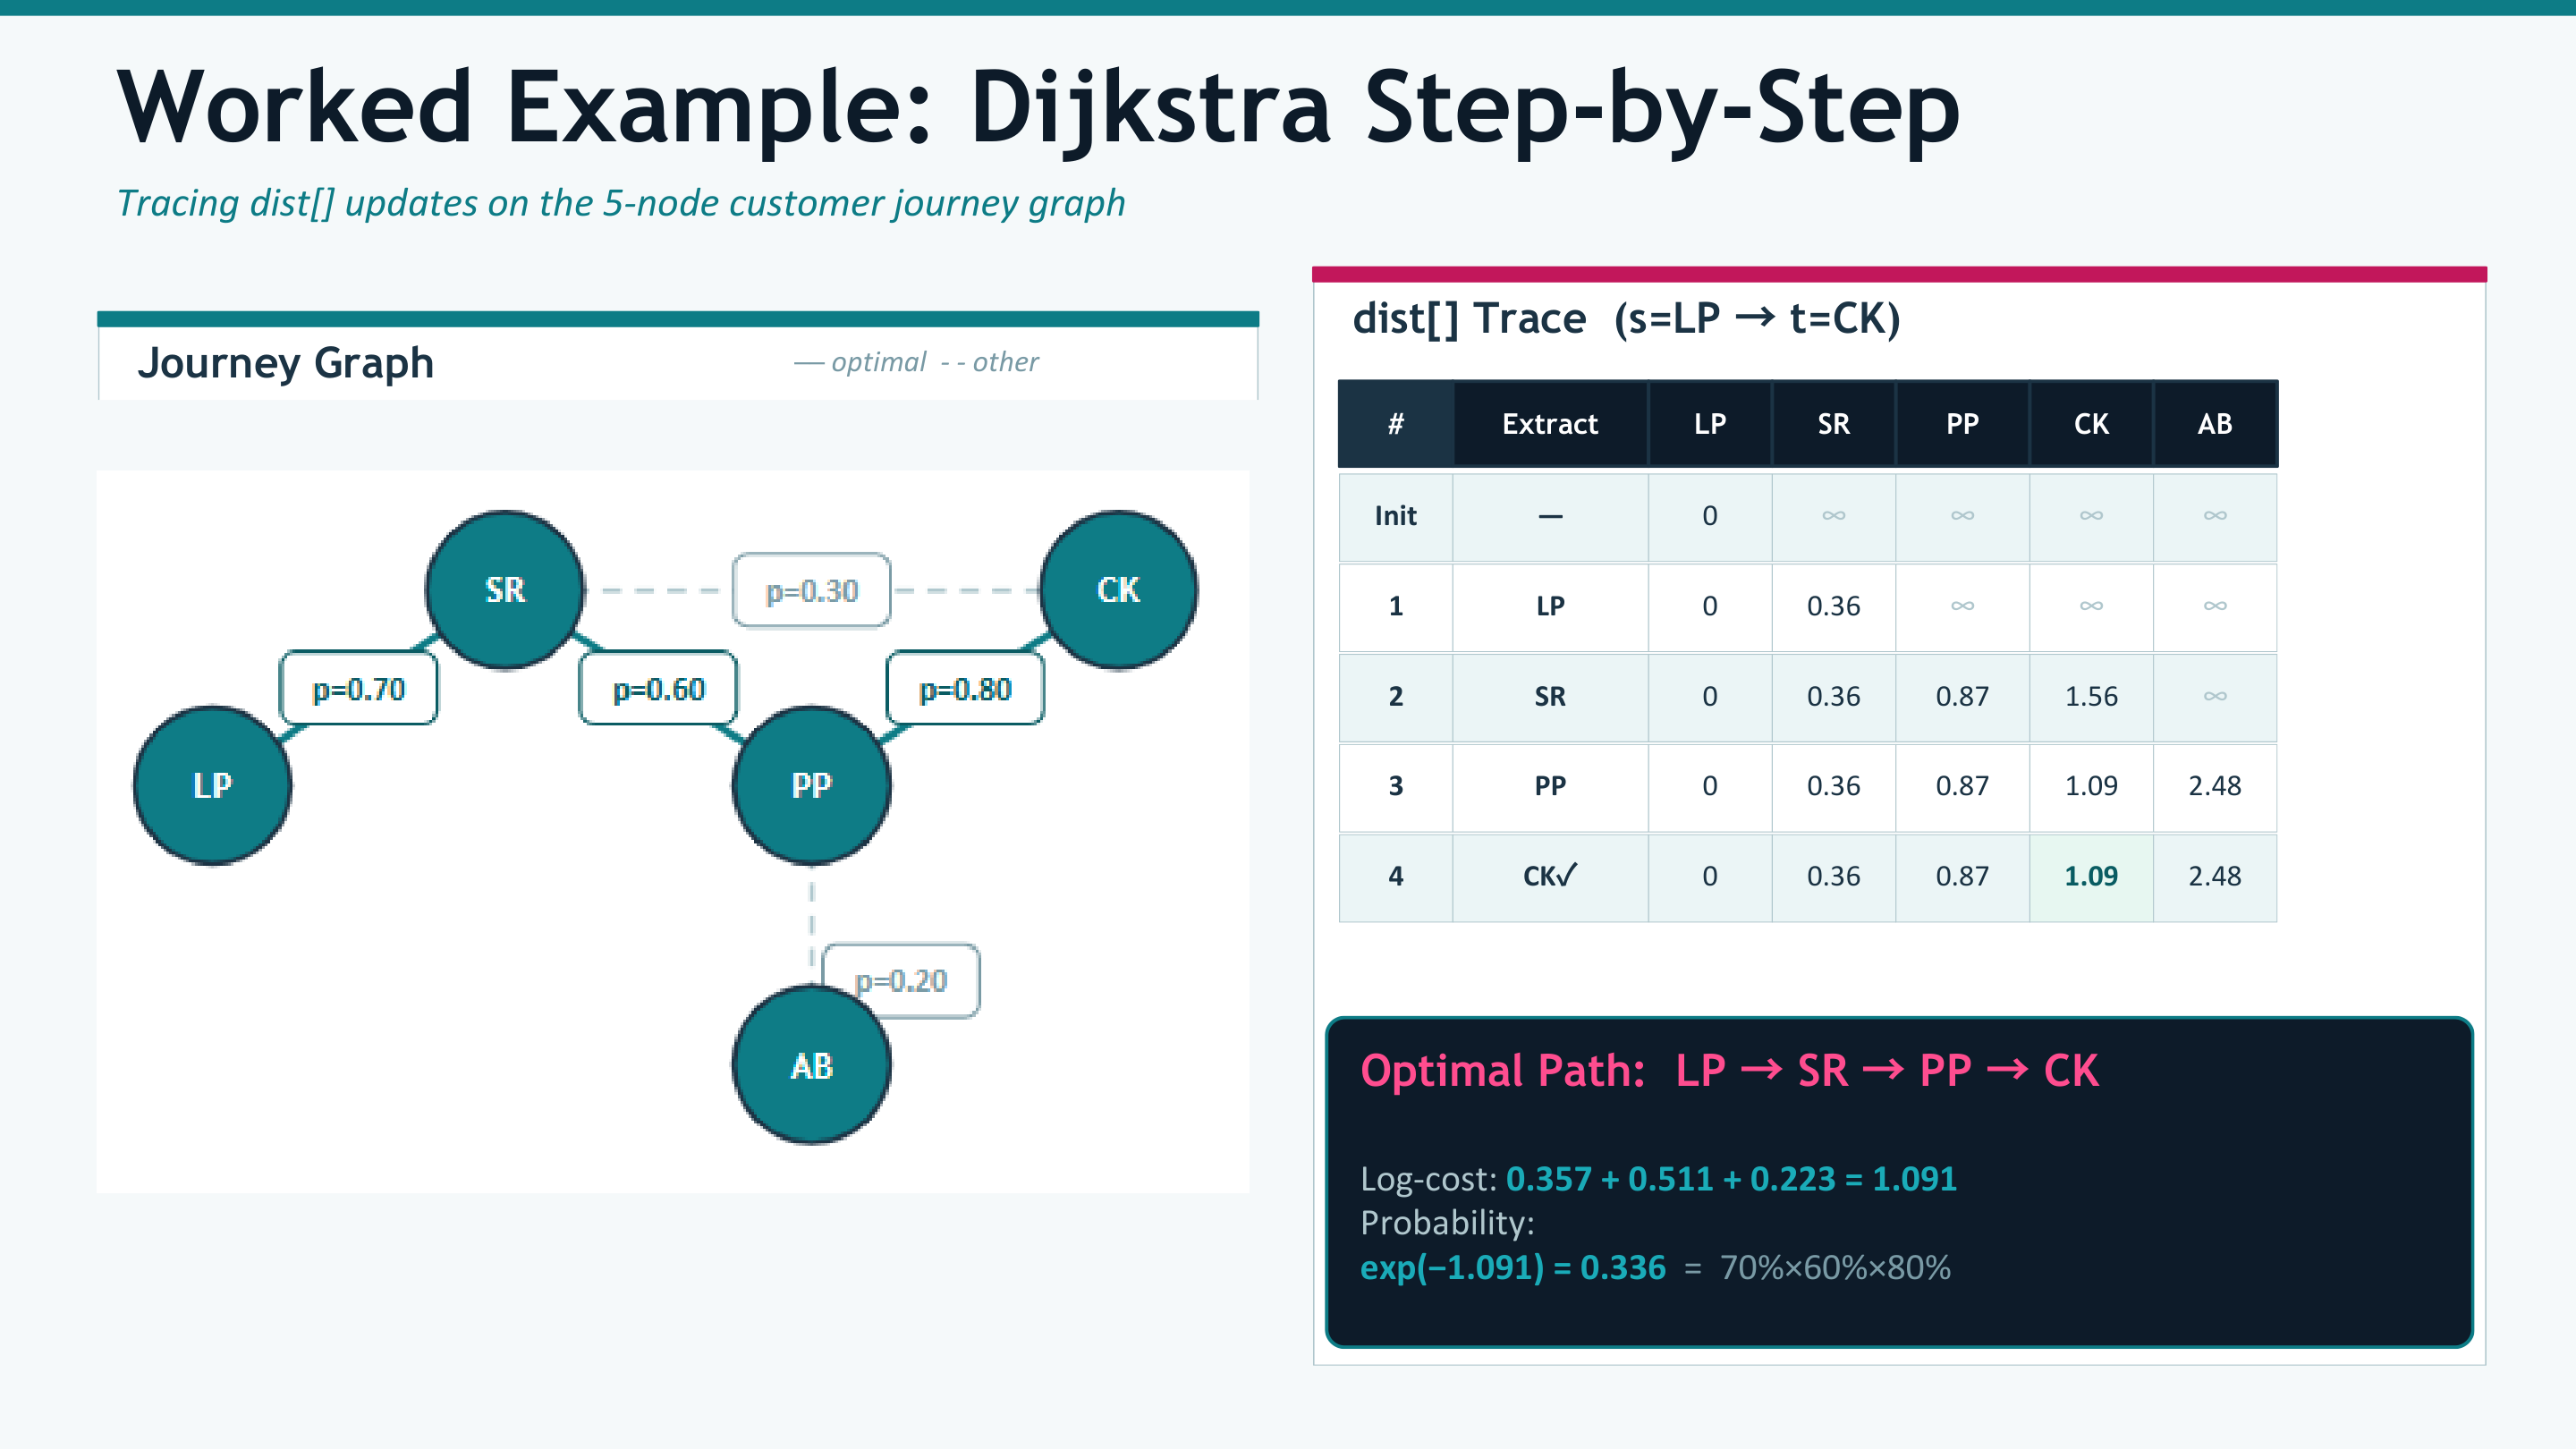
\includegraphics[width=0.92\textwidth]{worked_example}
\caption[Dijkstra step-by-step worked example]{Dijkstra step-by-step trace on the five-node customer journey graph ($s=\text{LP}$, $t=\text{CK}$). The left panel shows the graph with edge probabilities; the right panel tabulates the \texttt{dist[]} array after each node extraction. The optimal path LP$\to$SR$\to$PP$\to$CK is found with log-cost $1.091$ and probability $0.336$.}
\label{fig:worked_example}
\end{figure}

\subsection{Optimized Algorithm: Probability-Pruned Dijkstra (Approximation Technique)}

The proposed algorithm extends the baseline by introducing a \textbf{probability pruning threshold} $\tau \in (0, 1]$. This falls within the class of \textbf{approximation algorithms}~\citep{cormen2009}: it deliberately sacrifices worst-case optimality guarantees in exchange for improved practical runtime, while providing a controlled convergence guarantee ($\tau \to 0$ recovers exact optimality). The pruning is deterministic and parameter-controlled, distinguishing it from stochastic approximations such as Monte Carlo sampling or beam search. Any partial path whose cumulative probability falls below $\tau$ is pruned. In log-space, this is:

\[
\text{dist}[u] > -\log(\tau) = T
\]

\begin{tcolorbox}[title=Algorithm 2: Probability-Pruned Dijkstra]
\begin{lstlisting}
Initialize dist[v] = INF for all v in V
Initialize parent[v] = NIL for all v in V
dist[s] = 0
Insert (0, s) into priority queue Q
T = -log(tau)               // pruning threshold in log-space

While Q is not empty:
    (d, u) = Extract-Min(Q)
    if u == t: break
    if d > dist[u]: continue  // stale entry
    For each edge (u, v) with weight w = -log(p(u,v)):
        new_dist = dist[u] + w
        If new_dist > T: continue   // PRUNE: below probability tau
        If new_dist < dist[v]:
            dist[v] = new_dist
            parent[v] = u
            Insert (new_dist, v) into Q

Return dist[t], exp(-dist[t]), ReconstructPath(parent, s, t)
\end{lstlisting}
\end{tcolorbox}

\noindent\textbf{Worst-case time complexity:} $O(|E| \log |V|)$ (when $\tau \to 0$).\\
\textbf{Expected time complexity:} $O(|E'| \log |V|)$, $|E'| \leq |E|$.\\
\textbf{Space complexity:} $O(|V| + |E|)$.

\begin{figure}[h!]
\centering
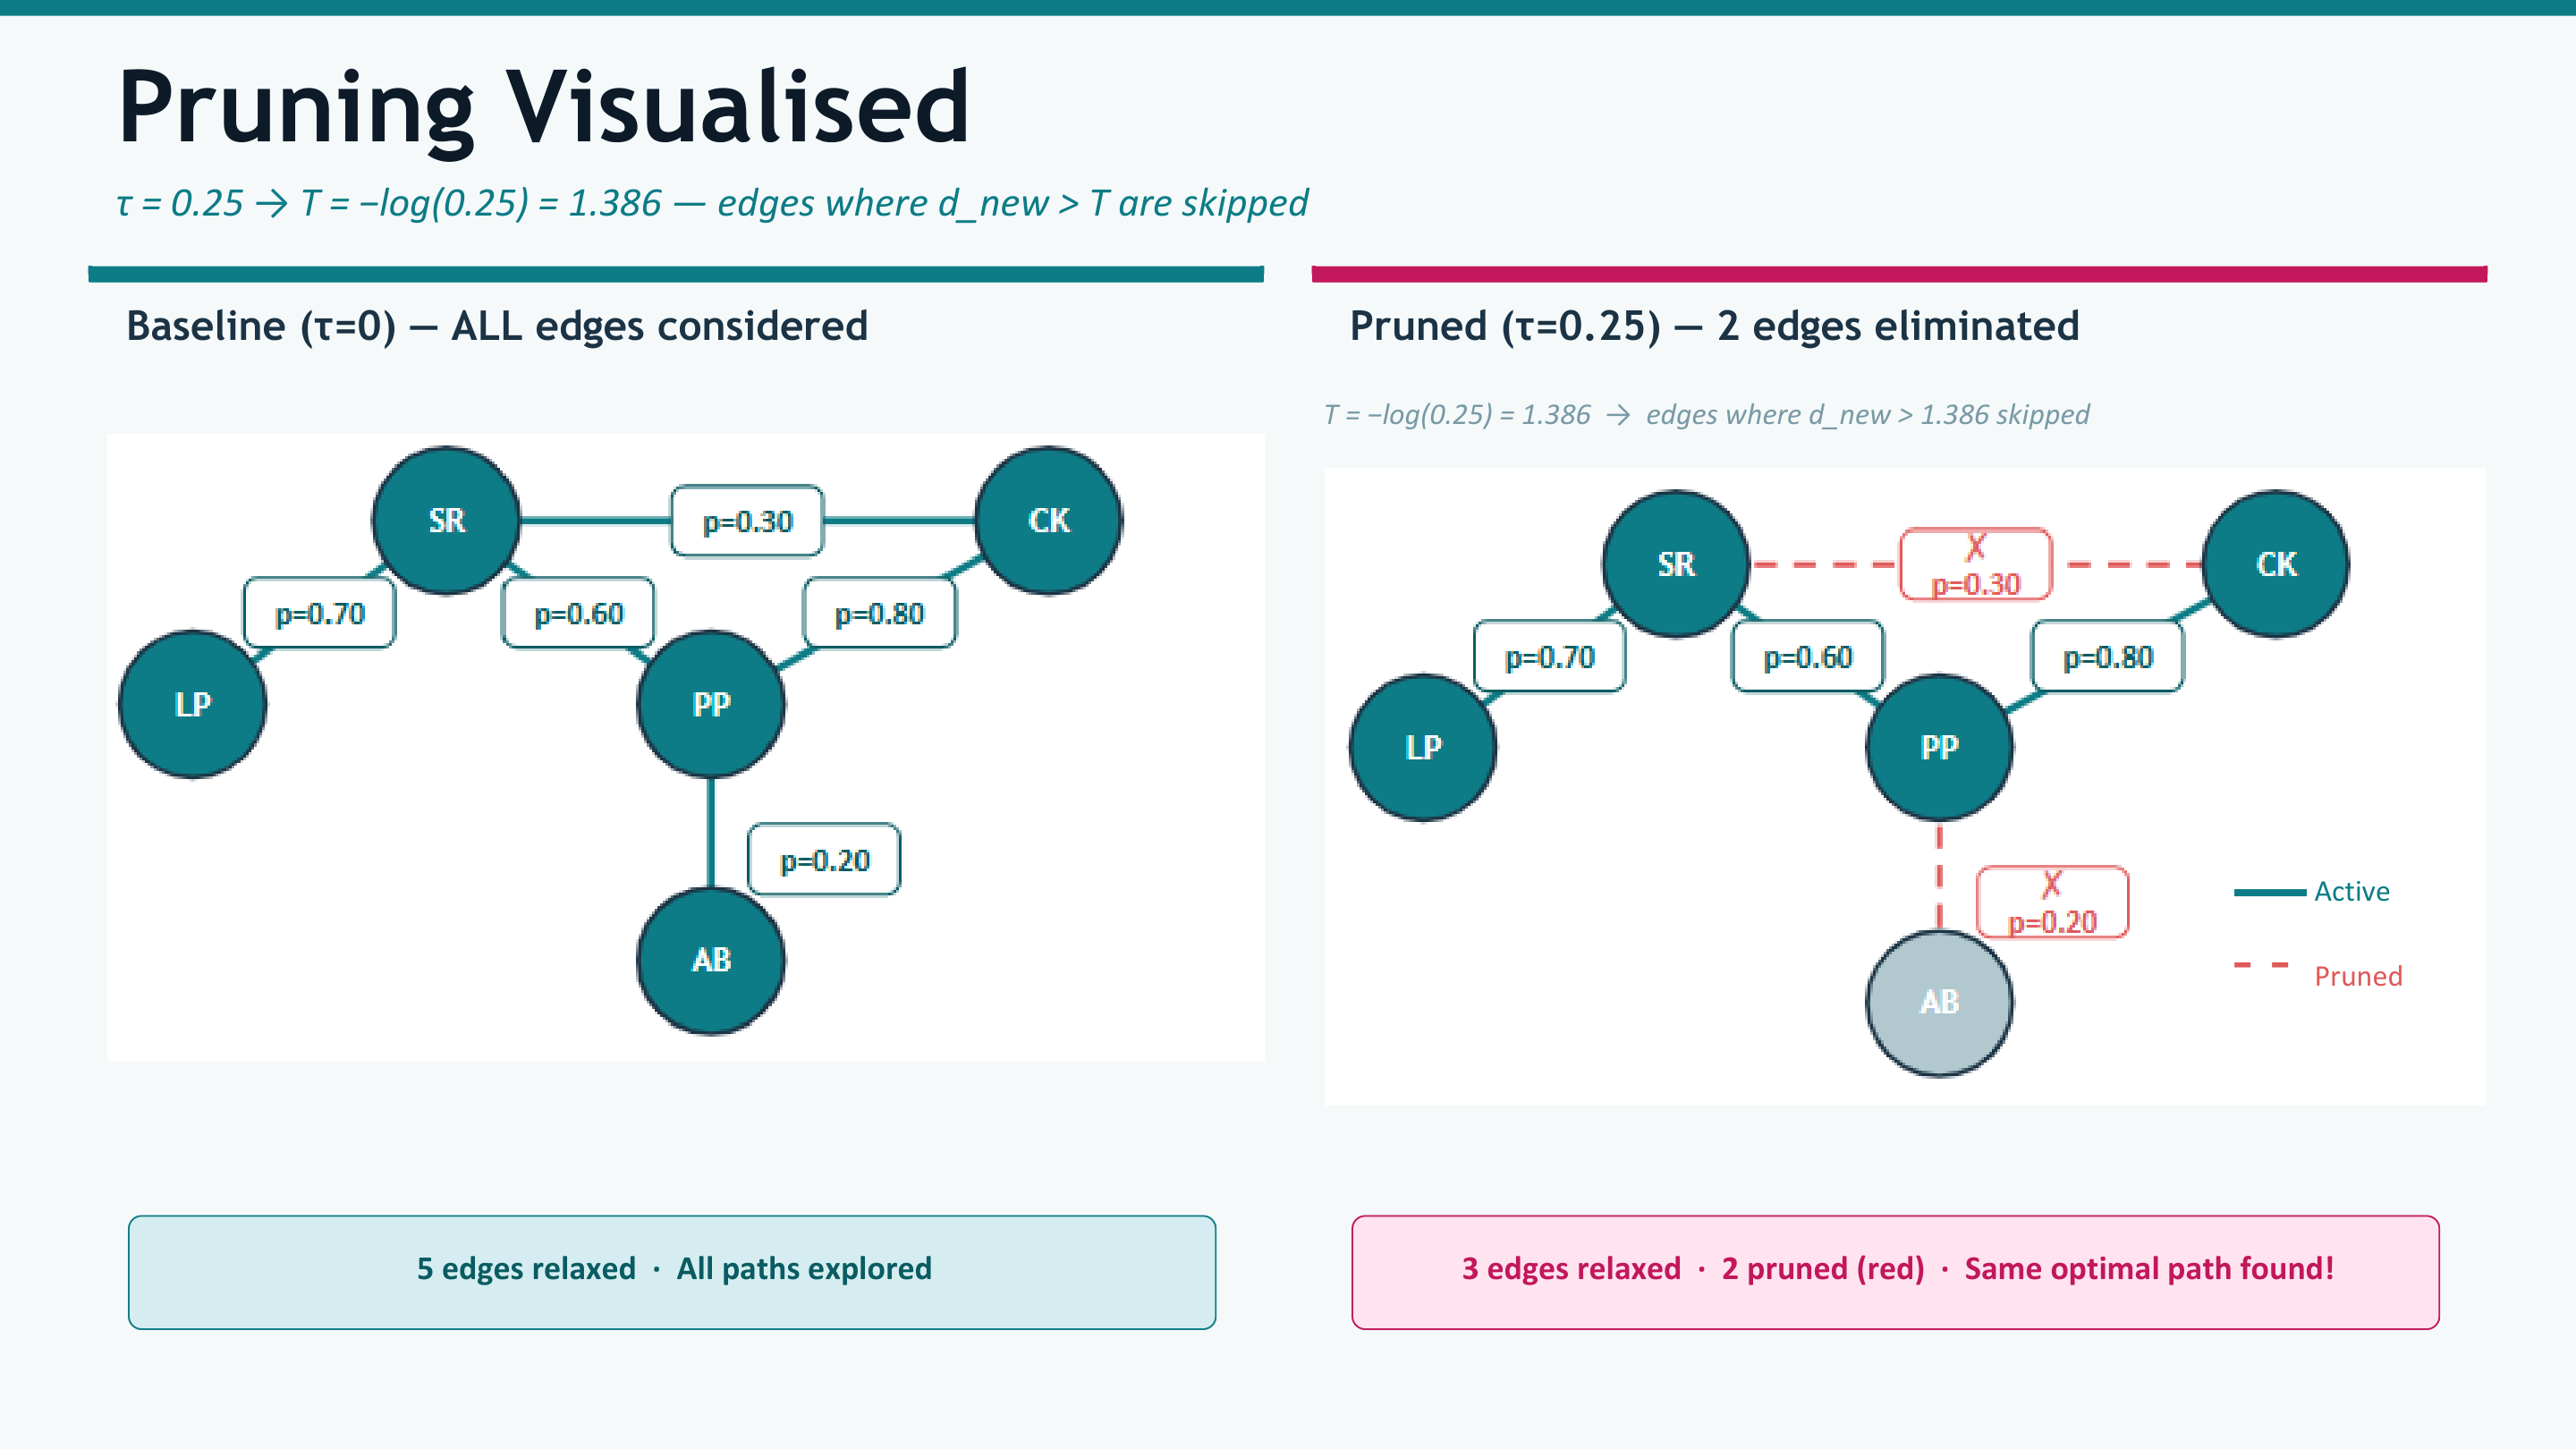
\includegraphics[width=0.92\textwidth]{pruning_visualised}
\caption[Pruning visualised: baseline vs.\ pruned Dijkstra on the example graph]{Pruning effect on the five-node customer journey graph with $\tau = 0.25$ ($T = -\log(0.25) = 1.386$). \textbf{Left:} Baseline Dijkstra relaxes all 5 edges. \textbf{Right:} Pruned Dijkstra eliminates 2 edges (dashed red) whose accumulated cost exceeds $T$---the SR$\to$CK shortcut and the PP$\to$AB branch---while still finding the same globally optimal path LP$\to$SR$\to$PP$\to$CK with only 3 edge relaxations.}
\label{fig:pruning_visualised}
\end{figure}

\subsection{Algorithm Comparison: Benefits and Drawbacks}
\label{sec:algocomparison}

Figure~\ref{fig:algo_flowchart} illustrates the decision-flow difference between both algorithms. In the baseline (left), every extracted node proceeds directly to neighbour relaxation. In the pruned variant (right), an extra threshold check $d_{\text{new}}>T=-\log(\tau)$ is inserted before each relaxation: edges exceeding the threshold are discarded (red PRUNE box), reducing the priority queue frontier and heap-operation overhead. Table~\ref{table:algo_compare} summarises the resulting trade-offs across eight criteria. The pruned algorithm will be compared against the baseline Dijkstra algorithm to measure runtime improvements and solution quality differences across all experimental configurations.

% ----------------------------------------------------------------
% FIGURE 3: Algorithm Comparison Flowchart
% ----------------------------------------------------------------
\begin{figure}[h!]
\centering
\begin{tikzpicture}[
    node distance=0.5cm and 1.6cm,
    startstop/.style={rectangle, rounded corners=8pt, minimum width=2.5cm, minimum height=0.7cm,
                      draw=black, thick, font=\small\bfseries, text centered},
    process/.style={rectangle, minimum width=2.5cm, minimum height=0.7cm,
                    draw=black, thick, font=\small, text centered},
    decision/.style={diamond, aspect=1.8, minimum width=2.8cm, minimum height=0.6cm,
                     draw=black, thick, font=\scriptsize\bfseries, text centered},
    prune/.style={rectangle, minimum width=2.5cm, minimum height=0.7cm,
                  draw=red!70!black, thick, fill=boxred, font=\small, text centered},
    arr/.style={-{Stealth[length=4pt]}, thick},
    lbl/.style={font=\scriptsize, fill=white, inner sep=1pt}
]

%--- LEFT COLUMN: Baseline Dijkstra ---
\node[startstop, fill=boxorange] (b_start) {Extract-Min$(Q)$};
\node[decision, below=0.5cm of b_start]  (b_tgt)   {$u = t$?};
\node[decision, below=0.7cm of b_tgt]    (b_stale)  {Stale?};
\node[process,  below=0.7cm of b_stale, fill=boxblue] (b_relax) {Relax neighbours};
\node[process,  below=0.5cm of b_relax, fill=boxblue] (b_push)  {Push to $Q$ if better};

% Straight-down arrows
\draw[arr] (b_start) -- (b_tgt);
\draw[arr] (b_tgt)   -- node[lbl,right]{No}  (b_stale);
\draw[arr] (b_stale) -- node[lbl,right]{No}  (b_relax);
\draw[arr] (b_relax) --                      (b_push);

% "Yes => Stop" from b_tgt:  go right, drop all the way to b_push level, merge in
\draw[arr] (b_tgt.east)
    -- ++(1.1,0)
    |- node[lbl, pos=0.25, right]{Yes $\Rightarrow$ \textbf{Stop}}
    (b_push.east);

% "Yes => Skip" from b_stale: go right, drop to b_relax level, merge in
\draw[arr] (b_stale.east)
    -- ++(0.8,0)
    |- node[lbl, pos=0.25, right]{Yes $\Rightarrow$ Skip}
    (b_relax.east);

\node[font=\small\bfseries, above=0.25cm of b_start, color=nodeorange] {Baseline Dijkstra};

%--- RIGHT COLUMN: Pruned Dijkstra ---
\node[startstop, fill=boxorange, right=3.8cm of b_start] (p_start) {Extract-Min$(Q)$};
\node[decision,  below=0.5cm of p_start]  (p_tgt)   {$u = t$?};
\node[decision,  below=0.7cm of p_tgt]    (p_stale)  {Stale?};
\node[decision,  below=0.7cm of p_stale]  (p_prune)  {$d_{\text{new}} > T$?};
\node[prune,     below=0.5cm of p_prune]  (p_skip)   {\textbf{PRUNE} (skip)};
\node[process,   right=1.3cm of p_prune, fill=boxblue] (p_relax)  {Relax edge};
\node[process,   below=0.5cm of p_skip,  fill=boxblue] (p_push)   {Push to $Q$ if better};

% Straight-down arrows
\draw[arr] (p_start) -- (p_tgt);
\draw[arr] (p_tgt)   -- node[lbl,right]{No}  (p_stale);
\draw[arr] (p_stale) -- node[lbl,right]{No}  (p_prune);
\draw[arr] (p_prune) -- node[lbl,left] {Yes} (p_skip);
\draw[arr] (p_skip)  --                      (p_push);

% "No" from p_prune goes right to p_relax, then p_relax drops down to p_push
\draw[arr] (p_prune.east) -- node[lbl,above]{No} (p_relax);
\draw[arr] (p_relax.south) |- (p_push.east);

% "Yes => Stop" from p_tgt: go right, drop all the way to p_push level
\draw[arr] (p_tgt.east)
    -- ++(1.4,0)
    |- node[lbl, pos=0.25, right]{Yes $\Rightarrow$ \textbf{Stop}}
    (p_push.east);

% "Yes => Skip" from p_stale: go right, drop to p_prune level
\draw[arr] (p_stale.east)
    -- ++(1.1,0)
    |- node[lbl, pos=0.25, right]{Yes $\Rightarrow$ Skip}
    (p_prune.east);

\node[font=\small\bfseries, above=0.25cm of p_start, color=nodegreen] {Pruned Dijkstra};
\end{tikzpicture}
\caption[Algorithm decision-flow comparison]{Decision-flow comparison of Baseline Dijkstra (left) and Pruned Dijkstra (right). The pruned variant adds a threshold check $d_{\text{new}}>T$ (red box); edges exceeding $T=-\log(\tau)$ are discarded without relaxation.}
\label{fig:algo_flowchart}
\end{figure}

\begin{table}[h!]
\centering
\renewcommand{\arraystretch}{1.3}
\begin{tabular}{@{}p{2.8cm}p{5.5cm}p{5.5cm}@{}}
\toprule
\textbf{Criterion} & \textbf{Baseline Dijkstra} & \textbf{Probability-Pruned Dijkstra} \\
\midrule
\textbf{Optimality} & Guaranteed globally optimal path for all $G$ with non-negative weights~\citep{dijkstra1959} & Guaranteed optimal only when $\tau = 0$; may return sub-optimal path for $\tau > 0$ \\[4pt]
\textbf{Time Complexity} & $O(|E|\log|V|)$ (worst and average case identical)~\citep{cormen2009} & $O(|E|\log|V|)$ worst case; $O(|E'|\log|V|)$ expected, $|E'| \leq |E|$ \\[4pt]
\textbf{Space Complexity} & $O(|V|+|E|)$ & $O(|V|+|E|)$ (unchanged) \\[4pt]
\textbf{Runtime on Large Graphs} & Can be slow on large, dense graphs due to full frontier expansion & Expected to be faster due to reduced frontier size and fewer heap operations \\[4pt]
\textbf{Parameter Tuning} & None required & Requires selection of $\tau$; too large risks missing optimal path \\[4pt]
\textbf{Approximation Bound} & Exact (no approximation) & No formal bound; trade-off evaluated empirically \\[4pt]
\textbf{Convergence} & Always finds optimal path if one exists & Converges to baseline as $\tau \to 0$~\citep{cormen2009} \\[4pt]
\textbf{Use Case} & Correctness-critical applications; small to medium graphs & Large graphs where approximation is acceptable; scalability-critical settings \\
\bottomrule
\end{tabular}
\caption[Algorithm comparison]{Comparison of Baseline and Pruned Dijkstra across key criteria. See Chapter~\ref{chap:complexity} for full complexity analysis.}
\label{table:algo_compare}
\end{table}

\section{Data Structures}

Figure~\ref{fig:data_structures} summarises the three complementary data structures used in both algorithms, along with their critical operation complexities. Each structure is chosen for a specific asymptotic property that directly contributes to the overall $O(|E|\log|V|)$ time bound.

\begin{figure}[h!]
\centering
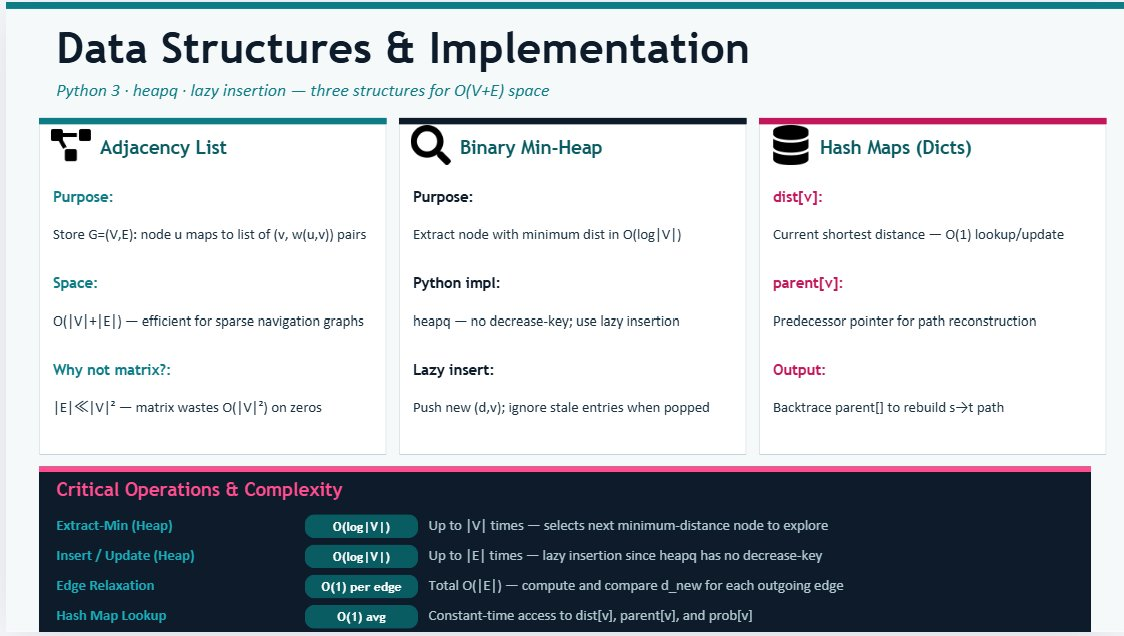
\includegraphics[width=0.95\textwidth]{data_structures}
\caption[Data structures and implementation overview]{Data structures and implementation overview for both algorithms. \textbf{Top row:} Adjacency List ($O(|V|+|E|)$ space, efficient for sparse graphs); Binary Min-Heap (Python \texttt{heapq} with lazy insertion, $O(\log|V|)$ extract-min and insert); Hash Maps (\texttt{dist[v]} and \texttt{parent[v]} with $O(1)$ average lookup). \textbf{Bottom panel:} Critical operation complexities --- Extract-Min $O(\log|V|)$; Insert/Update $O(\log|V|)$; Edge Relaxation $O(1)$ per edge; Hash Map Lookup $O(1)$ average.}
\label{fig:data_structures}
\end{figure}

\subsection{Adjacency List}

The directed graph will be stored as an adjacency list mapping each node $u$ to its outgoing neighbours and associated log-transformed weights. This ensures $O(|V|+|E|)$ space and efficient $O(\deg(u))$ neighbour iteration---both critical for sparse navigation graphs~\citep{cormen2009}.

\subsection{Binary Min-Heap (Priority Queue)}

A binary min-heap will serve as the priority queue, supporting~\citep{cormen2009,fredman1987fibonacci}:
\begin{itemize}
    \item \textbf{Extract-min:} $O(\log|V|)$, occurring up to $|V|$ times per run.
    \item \textbf{Insert:} $O(\log|V|)$, occurring up to $|E|$ times per run.
    \item \textbf{Edge Relaxation:} Computing updated log-distances and the pruning condition per edge; total cost $O(|E|)$ across the full traversal~\citep{cormen2009}.
    \item \textbf{Neighbour Iteration:} Iterating outgoing edges of each extracted node; total cost $O(|E|)$.
\end{itemize}

\subsection{Hash Maps (Dictionaries)}

Hash maps store \texttt{dist[v]} and \texttt{parent[v]} with $O(1)$ average-case access~\citep{cormen2009}.

\section{Complexity and Correctness}

Full complexity analysis is presented in Chapter~\ref{chap:complexity} and the correctness argument plan in Chapter~\ref{chap:correctness}. Briefly: both algorithms run in $O(|E|\log|V|)$ worst-case time and $O(|V|+|E|)$ space; the pruned algorithm reduces expected-case time to $O(|E'|\log|V|)$ with $|E'|\leq|E|$. Correctness of the baseline follows from the greedy invariant of Dijkstra's algorithm; the pruned variant converges to the baseline as $\tau\to 0$.

\section{Experimental Design}
\label{sec:expdesign}

\subsection{Simulation Environment}

All experiments will be implemented in Python using only standard libraries to ensure transparency of algorithmic implementation. Graphs will be represented using adjacency lists and priority queues will be implemented using Python's \texttt{heapq}. Runtime will be measured using \texttt{time.perf\_counter()} and memory usage tracked using \texttt{tracemalloc}. Each experiment configuration will be repeated at least 10 times with fixed random seeds to ensure reproducibility and fair comparison. Table~\ref{table:simenv} summarises the planned environment. Using only standard library components ensures that all algorithmic choices---data structures, timing, and memory profiling---are directly comparable across configurations without interference from third-party library overhead.

\begin{table}[h!]
\centering
\renewcommand{\arraystretch}{1.3}
\begin{tabular}{@{}ll@{}}
\toprule
\textbf{Component} & \textbf{Planned Specification} \\
\midrule
Programming Language & Python (standard library only) \\
Graph Representation & Adjacency list (\texttt{dict}) \\
Priority Queue & \texttt{heapq} (binary min-heap) \\
Runtime Measurement & \texttt{time.perf\_counter()} \\
Memory Measurement & \texttt{tracemalloc} peak allocation \\
Random Seeds & Fixed per configuration (for reproducibility) \\
Repetitions & $\geq 10$ runs per configuration \\
Graph Generator & Custom sparse graph generator (in-house) \\
\bottomrule
\end{tabular}
\caption[Planned simulation environment]{Planned simulation environment. All components use Python standard library only to ensure transparent, reproducible comparisons.}
\label{table:simenv}
\end{table}

\subsection{Evaluation Metrics}

Each experiment will record the following metrics across both algorithms and all input sizes:
\begin{itemize}
    \item \textbf{Execution Time (ms):} Wall-clock time measured with \texttt{time.perf\_counter()}.
    \item \textbf{Peak Memory Usage (MB):} Maximum resident memory during execution, measured with \texttt{tracemalloc}, capturing the practical space overhead of both algorithms across input sizes.
    \item \textbf{Nodes Explored:} Number of vertices extracted from the priority queue.
    \item \textbf{Edges Relaxed:} Total edge relaxation operations performed.
    \item \textbf{Path Probability $\Pi^*$:} Final cumulative probability $\prod_{(u,v)\in P^*} p(u,v)$.
    \item \textbf{Relative Optimality Gap:}
    \[
    \Delta = \frac{|\Pi^*_{\text{baseline}} - \Pi^*_{\text{proposed}}|}{\Pi^*_{\text{baseline}}} \times 100\%
    \]
    where $\Pi^*_{\text{baseline}}$ and $\Pi^*_{\text{proposed}}$ denote the path probabilities (scalar values in $[0,1]$) returned by the baseline and pruned algorithms respectively.
    \item \textbf{Max Frontier Size (MaxPQSize):} Maximum number of elements in the priority queue during execution.
\end{itemize}

\subsection{Experimental Parameters}

The following parameters will be varied systematically:
\begin{itemize}
    \item \textbf{Input Size $|V|$:} 1,000 (small), 5,000--10,000 (medium), up to 50,000 (large).
    \item \textbf{Edge Density:} Average out-degree $\bar{d} \in \{2, 5, 10\}$ edges per node.
    \item \textbf{Probability Distribution:} Uniform $\mathcal{U}(0,1]$ vs.\ skewed (power-law with exponent $\alpha = 2$).
    \item \textbf{Pruning Threshold $\tau$:} $\{0,\; 0.001,\; 0.01,\; 0.05,\; 0.1,\; 0.5\}$.

    \item \textbf{Graph Type:} Erd\H{o}s--R\'enyi sparse random graphs and layered/stage-based customer-journey graphs.
    
\end{itemize}



\subsection{Experimental Controls}

\begin{itemize}
    \item Both algorithms run on identical graph instances (same seed, same generated graph).
    \item Single-threaded execution on a dedicated machine to eliminate scheduling noise.
    \item Each configuration repeated $\geq 10$ times; mean and standard deviation reported.
    \item Memory measured independently per run using \texttt{tracemalloc.get\_traced\_memory()}.
\end{itemize}

\subsection{Risks and Fallback Plan}

Main technical risks: (1) over-aggressive pruning at high $\tau$ eliminating near-optimal paths; (2) dense graphs limiting pruning benefit; (3) uniform probability distributions offering little search-space reduction; (4) large graphs approaching RAM limits.

Should pruning provide minimal runtime or memory improvement, the project will pivot to a detailed scalability analysis of the baseline, conduct a threshold sensitivity study, and present comparative results identifying when pruning is and is not effective. The minimum acceptable outcome is a validated baseline implementation, formal complexity analysis, and an empirical baseline-vs-pruned comparison demonstrating correctness, scalability, and reproducibility.

    \chapter{CORRECTNESS ARGUMENT PLAN}\label{chap:correctness}

This chapter outlines the approach that will be used to argue the correctness of both the baseline Dijkstra algorithm and the probability-pruned Dijkstra algorithm. Since this is a proposal, full formal proofs are not presented; instead, the key invariants, proof strategies, and verification plans are identified.

\section{Correctness of the Log-Probability Transformation}

\textbf{Claim:} The path $P^*$ that minimizes $\sum_{(u,v)\in P} -\log\,p(u,v)$ is identical to the path that maximizes $\prod_{(u,v)\in P} p(u,v)$.

\textbf{Proof sketch:} The negative logarithm $-\log(\cdot)$ is a strictly monotone decreasing function on $(0,1]$~\citep{cormen2009}. Therefore, for any two paths $P_1$ and $P_2$:
\[
\prod_{(u,v)\in P_1} p(u,v) \;>\; \prod_{(u,v)\in P_2} p(u,v)
\;\iff\;
\sum_{(u,v)\in P_1} -\log\,p(u,v) \;<\; \sum_{(u,v)\in P_2} -\log\,p(u,v)
\]
This follows directly from applying $-\log$ to both sides and reversing the inequality (since $-\log$ is decreasing). The transformation is therefore \emph{order-preserving}: the ranking of paths by probability is identical to the ranking by log-cost, so maximizing probability is equivalent to minimizing log-cost~\citep{manning2008nlp,viterbi1967error}. Non-negativity of weights ($w(u,v) \geq 0$ since $p(u,v) \in (0,1]$) will be verified formally during implementation.

\section{Correctness of Baseline Dijkstra}\label{sec:correctness_baseline}

\textbf{Algorithm paradigm:} Dijkstra's algorithm is a greedy algorithm~\citep{cormen2009}. Its correctness rests on a \textbf{greedy invariant} maintained throughout execution.

\textbf{Key invariant:} At any point during the algorithm, for every node $u$ that has been extracted from the priority queue, $\text{dist}[u]$ is the true shortest-path distance from $s$ to $u$ in the transformed graph.

\textbf{Proof plan:} The invariant will be established by induction on the number of extracted nodes~\citep{cormen2009,dijkstra1959}:
\begin{enumerate}
    \item \textbf{Base case:} The source node $s$ is extracted first with $\text{dist}[s] = 0$, which is trivially correct.
    \item \textbf{Inductive step:} Assume all previously extracted nodes satisfy the invariant. When node $u$ is extracted, suppose for contradiction that there exists a shorter path $s \leadsto u$ through some unextracted node $x$. Since all edge weights are non-negative, the distance through $x$ to $u$ must be $\geq \text{dist}[x] \geq \text{dist}[u]$ (by the priority queue ordering), which contradicts the assumption. Therefore $\text{dist}[u]$ is optimal at extraction~\citep{cormen2009}.
    \item \textbf{Termination:} The algorithm terminates when the target $t$ is extracted or the queue is empty, at which point the invariant guarantees optimality of $\text{dist}[t]$.
\end{enumerate}

\textbf{Correctness of path recovery:} The path $P^*$ is reconstructed from the \texttt{parent} array by backtracking from $t$ to $s$. Correctness of this reconstruction follows from the fact that each parent pointer is set only when a strictly shorter path is found, so the chain of parent pointers forms a valid shortest-path tree~\citep{cormen2009}.

\section{Correctness of Probability-Pruned Dijkstra}

\textbf{Claim for $\tau = 0$:} When $\tau = 0$, $T = -\log(0^+) = +\infty$, so the pruning condition $\text{dist}[u] > T$ is never triggered and the algorithm is identical to the baseline. Full correctness follows from Section~\ref{sec:correctness_baseline}.

\textbf{Convergence claim for $\tau \to 0$:} As $\tau$ decreases toward 0, $T = -\log(\tau)$ increases toward $+\infty$, and the pruning condition eliminates progressively fewer edges. In the limit, all edges are explored and the result converges exactly to the baseline optimal solution.

\textbf{Approximation behavior for $\tau > 0$:} For $\tau > 0$, the algorithm may prune the optimal path if its cumulative probability falls below $\tau$. This is an intentional approximation: if the optimal path has probability $\Pi^* < \tau$, then the algorithm may return a sub-optimal path or report failure. This behavior will be empirically characterized through the optimality gap metric $\Delta$ defined in Section~\ref{sec:expdesign}.

\textbf{Proof plan for approximation:} No formal approximation bound is claimed for $\tau > 0$; correctness in the approximate sense will be established empirically by comparing pruned outputs to baseline outputs across all experimental configurations (Section~\ref{sec:expdesign}).

\section{Verification Strategy}

All correctness claims will be validated through:
\begin{enumerate}
    \item \textbf{Manual trace:} On the small example graph (Figure~\ref{fig:journey_graph}), both algorithms will be traced step-by-step to verify that $\text{dist}[\text{CK}] = -\log(0.7) - \log(0.6) - \log(0.8) \approx 1.091$ and that the path LP$\to$SR$\to$PP$\to$CK is returned.
    \item \textbf{Invariant checking:} An optional debug mode will assert the greedy invariant after every extraction during testing.
    \item \textbf{Convergence testing:} The pruned algorithm will be run with $\tau \in \{0.5, 0.1, 0.01, 0.001, 0\}$ on the same graph instances to confirm monotone convergence to the baseline solution.
    \item \textbf{Probability consistency check:} For all returned paths, $\exp(-C^*)$ will be verified to equal $\prod_{(u,v)\in P^*} p(u,v)$ within floating-point precision.
    \item \textbf{Edge case testing:} Disconnected graphs (no $s$-to-$t$ path), single-node graphs, and graphs with probability-1 edges will be tested.
\end{enumerate}

    \chapter{COMPLEXITY ANALYSIS PLAN}\label{chap:complexity}

This chapter presents the expected time and space complexity of both algorithms and describes the methodology by which these bounds will be derived and empirically validated.

\section{Analytical Methodology}

The complexity of both algorithms will be analyzed using the standard \textbf{operation-counting} approach~\citep{cormen2009}:
\begin{enumerate}
    \item Identify all operations performed by the algorithm (heap insertions, extractions, edge relaxations, comparisons).
    \item Count the maximum number of times each operation is performed as a function of $|V|$ and $|E|$.
    \item Multiply by the cost of each operation (determined by the data structure) and sum to obtain the total complexity.
    \item Verify the asymptotic bound holds empirically by plotting runtime against $|V|$ and $|E|$ on log-log axes and checking that the slope matches the theoretical exponent.
\end{enumerate}

\section{Time Complexity}

\subsection{Baseline Dijkstra}

The time complexity analysis proceeds as follows~\citep{cormen2009,dijkstra1959}:

\begin{enumerate}
    \item \textbf{Initialization:} Setting \texttt{dist[v] = INF} and \texttt{parent[v] = NIL} for all $v \in V$ costs $O(|V|)$.
    \item \textbf{Priority queue insertions:} Each node is inserted at most once initially, and re-inserted (lazy) at most once per incoming edge. Total insertions $\leq |V| + |E|$. Each insertion costs $O(\log|V|)$ (binary heap sift-up). Total: $O(|E|\log|V|)$.
    \item \textbf{Extract-min operations:} Each node may be extracted multiple times (due to lazy insertion), but each extraction is $O(\log|V|)$. Total extractions $\leq |V| + |E|$. Total: $O(|E|\log|V|)$.
    \item \textbf{Edge relaxations:} For each extracted node $u$, all $\deg(u)$ outgoing edges are examined. Across the full algorithm, each edge is relaxed at most once: $\sum_{u\in V} \deg(u) = |E|$. Each relaxation costs $O(1)$ (comparison and hash map lookup). Total: $O(|E|)$.
\end{enumerate}

\noindent\textbf{Total time complexity:} $O(|E|\log|V|)$, dominated by heap operations~\citep{cormen2009}.

In sparse graphs where $|E| = O(|V|)$, this simplifies to $O(|V|\log|V|)$.

\textit{Note:} A Fibonacci heap would reduce the bound to $O(|E| + |V|\log|V|)$~\citep{fredman1987fibonacci}, but binary heaps are used here for practical simplicity and lower constant factors.

\subsection{Probability-Pruned Dijkstra}

\begin{enumerate}
    \item \textbf{Worst case ($\tau = 0$):} No edges are pruned; the algorithm is identical to the baseline. Worst-case time complexity: $O(|E|\log|V|)$.
    \item \textbf{Expected case ($\tau > 0$):} Let $|E'| \leq |E|$ denote the number of edges not pruned. Edges $(u,v)$ for which $\text{dist}[u] + w(u,v) > T$ are skipped in $O(1)$ without a heap insertion. The expected complexity is $O(|E'|\log|V|)$, where $|E'|$ depends on $\tau$ and the probability distribution.
    \item \textbf{Analysis of $|E'|$:} The fraction of edges pruned will be characterized empirically as a function of $\tau$, graph size $|V|$, and probability distribution (uniform vs.\ skewed). The expected pruning ratio $1 - |E'|/|E|$ will be plotted against $\tau$ to empirically characterize how aggressively each configuration benefits from pruning.
\end{enumerate}

\subsection{Empirical Validation Plan}

To verify that the theoretical bounds hold in practice, the following procedure will be followed:
\begin{itemize}
    \item For each graph size $|V| \in \{1{,}000,\;5{,}000,\;10{,}000,\;50{,}000\}$, measure mean execution time $T(|V|)$.
    \item Plot $\log T$ vs.\ $\log|V|$ (for sparse graphs where $|E| \propto |V|$) and verify slope $\approx 1$ (linear in $|V|\log|V|$).
    \item For the pruned algorithm, additionally plot $T_{\text{pruned}}$ vs.\ $|E'|/|E|$ to confirm that runtime scales proportionally to the fraction of edges explored.
\end{itemize}

\section{Space Complexity}

Both algorithms use the following data structures:

\begin{table}[h!]
\centering
\renewcommand{\arraystretch}{1.3}
\begin{tabular}{@{}lll@{}}
\toprule
\textbf{Data Structure} & \textbf{Space} & \textbf{Purpose} \\
\midrule
Adjacency list & $O(|V|+|E|)$ & Graph representation \\
Distance array \texttt{dist[v]} & $O(|V|)$ & Shortest path estimates \\
Parent array \texttt{parent[v]} & $O(|V|)$ & Path reconstruction \\
Priority queue (heap) & $O(|V|+|E|)$ worst case & Node ordering \\
\midrule
\textbf{Total} & $\mathbf{O(|V|+|E|)}$ & \\
\bottomrule
\end{tabular}
\caption[Space complexity breakdown]{Space complexity breakdown. Total is $O(|V|+|E|)$; in sparse graphs ($|E|=O(|V|)$) this reduces to $O(|V|)$ in practice.}
\label{table:space_complexity}
\end{table}

As shown in Table~\ref{table:space_complexity}, the dominant terms are the adjacency list and the priority queue, both $O(|V|+|E|)$. In the sparse graphs used in this project ($|E|=O(|V|)$), the total space simplifies to $O(|V|)$ in practice. Crucially, the pruning threshold $\tau$ adds no asymptotic space overhead: no additional arrays or data structures are required beyond those of the baseline algorithm.

\subsection{Empirical Memory Validation Plan}

Peak memory usage will be measured using Python's \texttt{tracemalloc} module across all input sizes. The expected behavior is:
\begin{itemize}
    \item Memory should grow approximately linearly with $|V|$ for sparse graphs (confirming $O(|V|)$ practical space).
    \item The pruned algorithm should exhibit lower peak priority queue memory due to fewer heap insertions, even though the asymptotic bound is the same.
    \item Memory results will be plotted against $|V|$ and compared to the theoretical $O(|V|+|E|)$ bound to confirm agreement.
\end{itemize}

\section{Summary of Expected Complexity}

Table~\ref{table:complexity_summary} summarises the time and space complexity for all three configurations.

\begin{table}[h!]
\centering
\renewcommand{\arraystretch}{1.4}
\begin{tabular}{@{}lccc@{}}
\toprule
\textbf{Algorithm} & \textbf{Time (worst)} & \textbf{Time (expected)} & \textbf{Space} \\
\midrule
Baseline Dijkstra & $O(|E|\log|V|)$ & $O(|E|\log|V|)$ & $O(|V|+|E|)$ \\
Pruned Dijkstra ($\tau=0$) & $O(|E|\log|V|)$ & $O(|E|\log|V|)$ & $O(|V|+|E|)$ \\
Pruned Dijkstra ($\tau>0$) & $O(|E|\log|V|)$ & $O(|E'|\log|V|)$, $|E'|\leq|E|$ & $O(|V|+|E|)$ \\
\bottomrule
\end{tabular}
\caption[Complexity summary]{Time and space complexity summary. Pruning reduces expected-case time to $O(|E'|\log|V|)$ with $|E'|\leq|E|$; worst-case and space bounds are unchanged.}
\label{table:complexity_summary}
\end{table}

When $\tau=0$ the pruned algorithm is identical to the baseline in all respects. For $\tau>0$, the worst-case bound is unchanged because in the worst case no path exceeds the threshold and all edges are processed. The practical benefit materialises in the expected case: edges whose accumulated log-cost exceeds $T=-\log(\tau)$ are skipped, reducing the effective edge count from $|E|$ to $|E'|\leq|E|$ and shrinking priority queue operations accordingly. These theoretical bounds will be validated empirically in Chapter~\ref{chap:results}.

Figure~\ref{fig:complexity_overview} summarises the full complexity and correctness properties of both algorithms in a side-by-side comparison, including the convergence guarantee and fallback strategy.

\begin{figure}[h!]
\centering
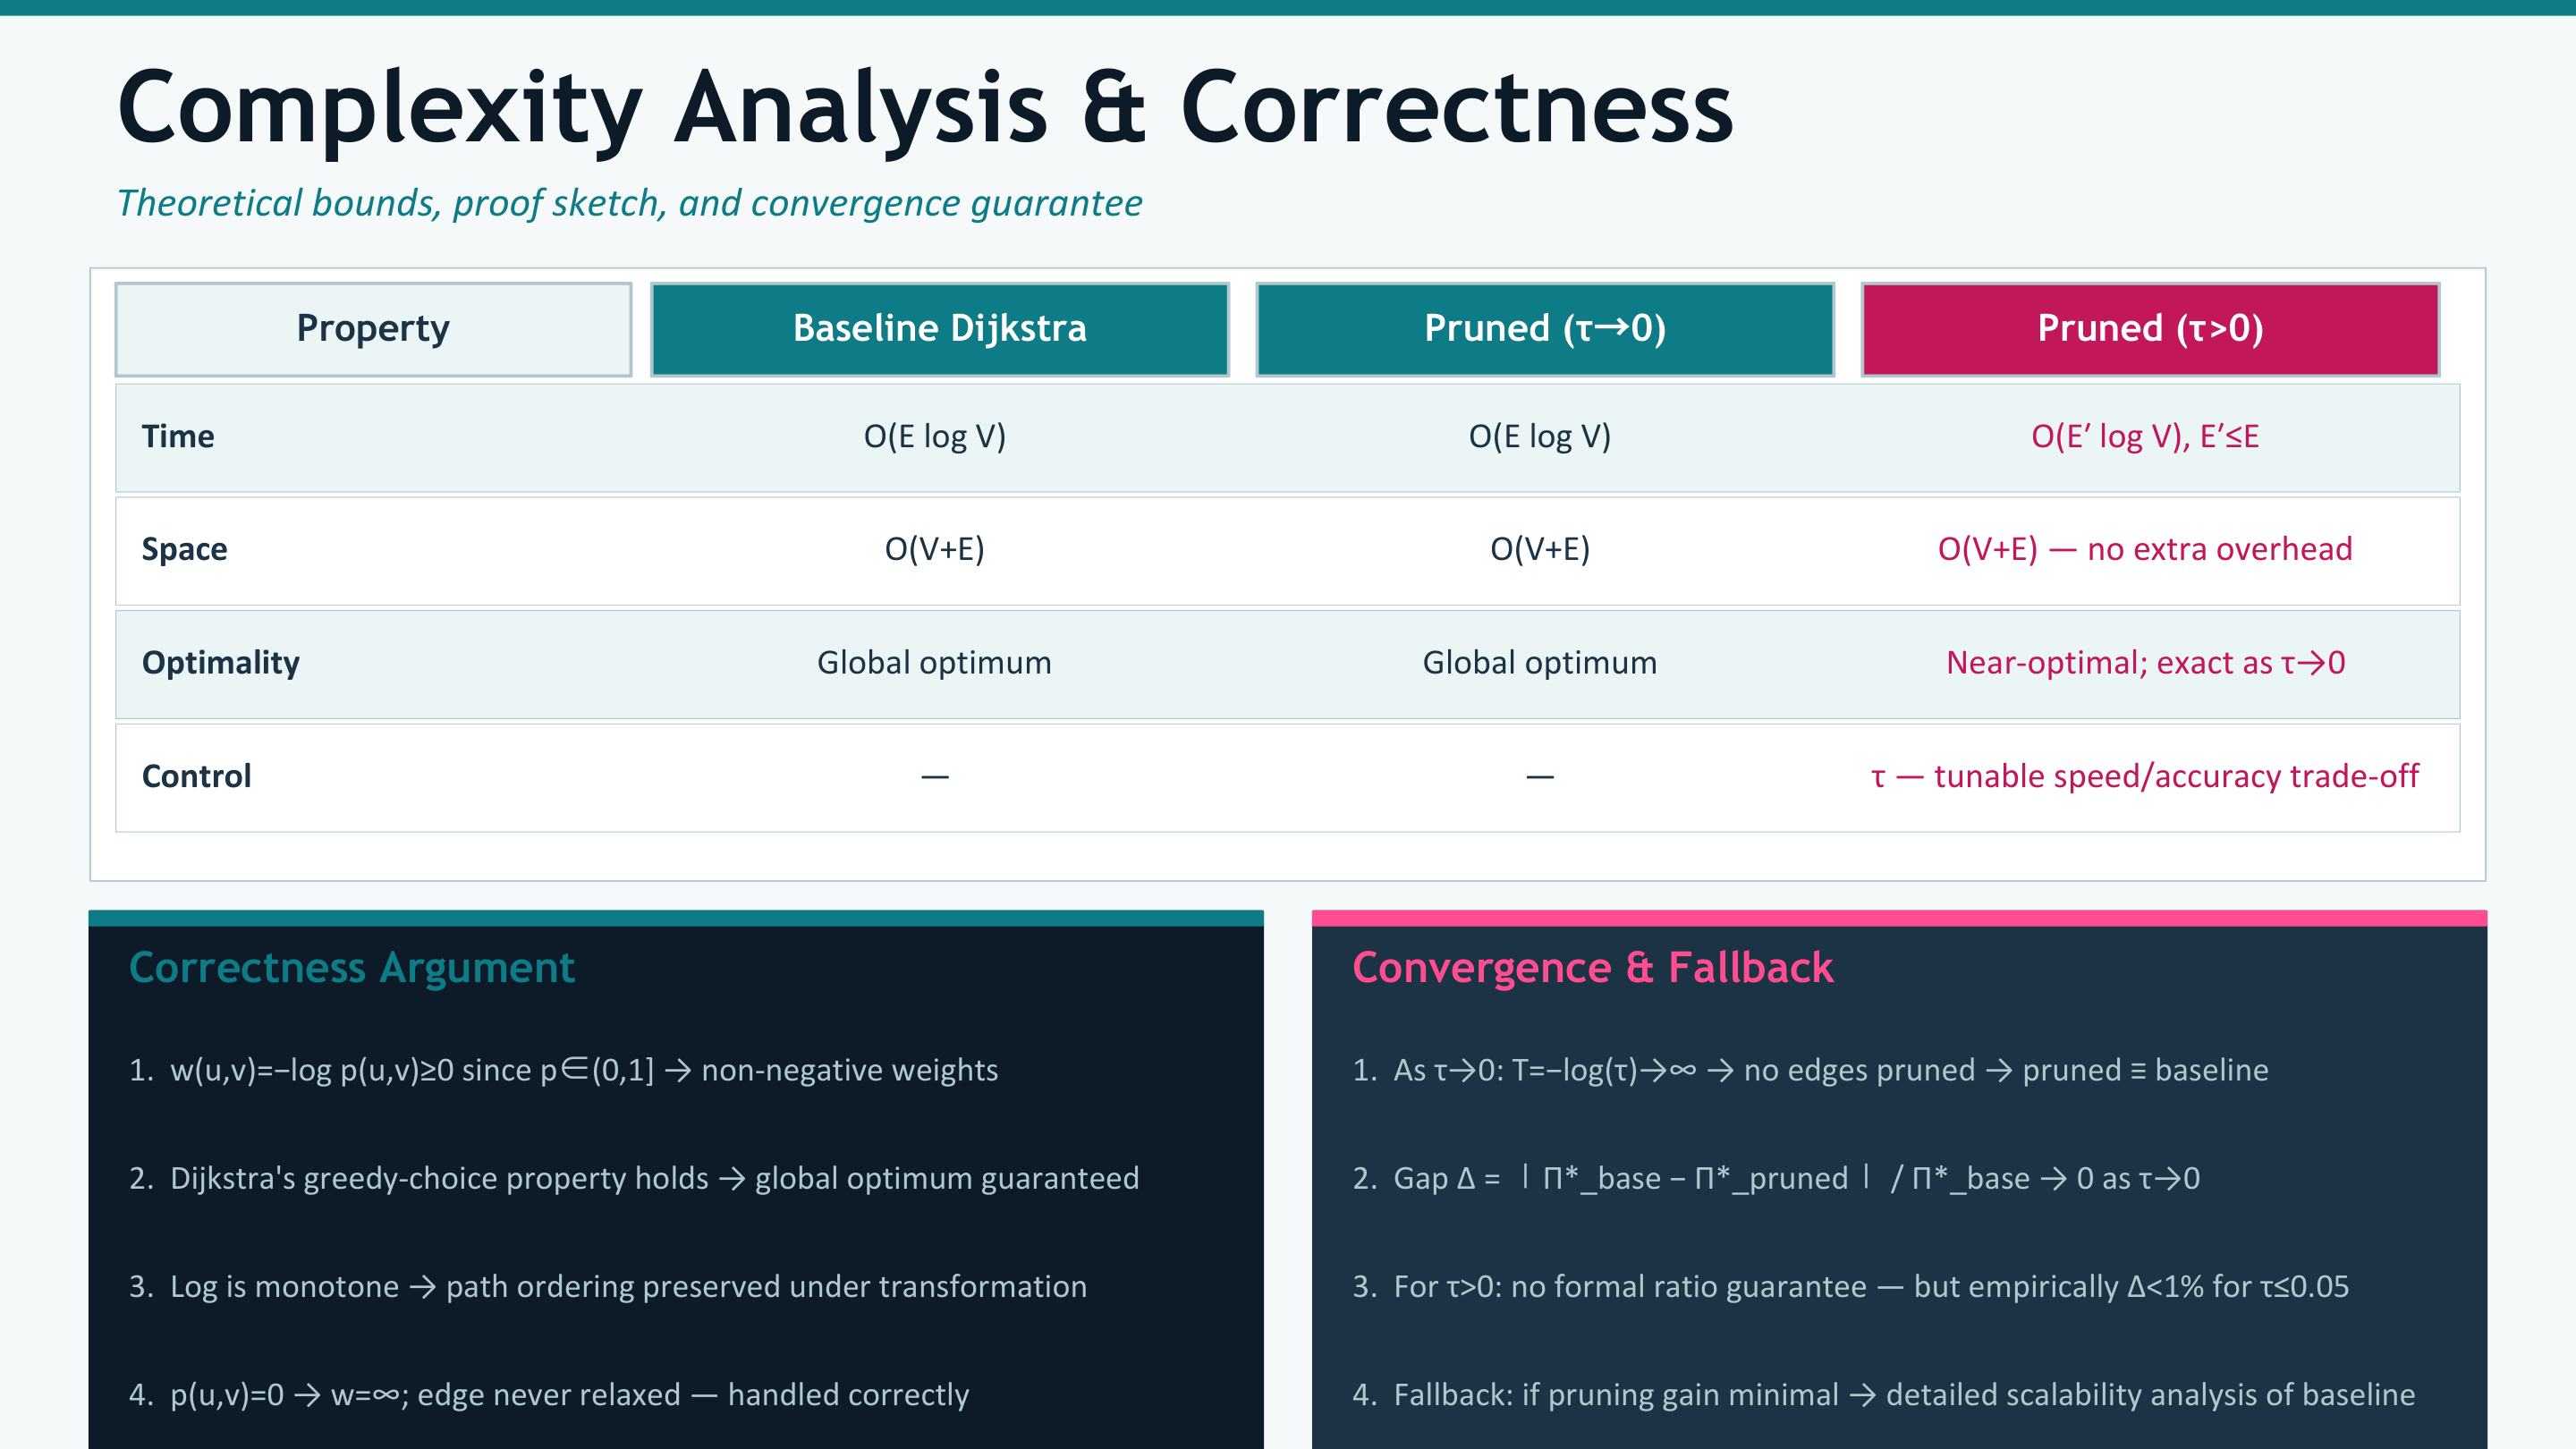
\includegraphics[width=0.95\textwidth]{complexity_table}
\caption[Complexity and correctness summary for both algorithms]{Summary of complexity and correctness properties. The upper table compares Time, Space, Optimality, and Control properties across three configurations (Baseline, Pruned $\tau\to0$, Pruned $\tau>0$). The lower panels give the four-point correctness argument (non-negative weights, greedy-choice invariant, monotone log-transform, zero-probability handling) and the four-point convergence guarantee ($\tau\to0$ recovers baseline; gap $\Delta\to0$; empirical $\Delta<1\%$ for $\tau\leq0.05$; fallback to baseline scalability analysis if pruning gain is minimal).}
\label{fig:complexity_overview}
\end{figure}

    \chapter{EXPECTED CONTRIBUTIONS AND PRELIMINARY RESULTS}\label{chap:results}

\section{Overview}

This chapter outlines the results that are anticipated upon completion of the experimental evaluation. Both the baseline Dijkstra algorithm and the proposed probability-pruned Dijkstra algorithm will be evaluated across synthetic graphs of varying sizes, edge densities, and probability distributions, with multiple values of the pruning threshold $\tau$. All results will be averaged over at least 10 independent runs per configuration, with standard deviation reported to characterize variance.

\section{Correctness Validation}

\subsection{Baseline Correctness}

The baseline Dijkstra implementation is expected to return the globally optimal path on all tested instances. The returned path probability $\exp(-\text{dist}[t])$ should match the product of edge probabilities $\prod_{(u,v)\in P^*} p(u,v)$ exactly, confirming numerical correctness of the log-space transformation.

\subsection{Convergence of Pruned Algorithm}

As $\tau \to 0$, the pruned algorithm is expected to converge to the baseline solution on all tested graph instances. At $\tau = 0$ (no pruning), both algorithms should return identical paths and probabilities, with any runtime difference attributable solely to the overhead of the additional pruning condition check. This will validate the theoretical convergence guarantee.

\section{Runtime Performance}

\subsection{Scalability with Graph Size}

Table~\ref{table:runtime} shows the placeholder structure for mean runtime and peak memory results across all graph sizes. Each column records the mean over $\geq10$ runs at fixed random seeds: execution time in milliseconds for each algorithm, speedup (Baseline / Pruned), and peak heap allocation in MB measured by \texttt{tracemalloc}. The pruned variant is run with $\tau=0.01$.

\begin{table}[h!]
\centering
\resizebox{\textwidth}{!}{%
\begin{tabular}{@{}lrrrrr@{}}
\toprule
\textbf{Graph Size ($|V|$)} & \textbf{Baseline (ms)} & \textbf{Pruned (ms)} & \textbf{Speedup} & \textbf{Baseline Mem (MB)} & \textbf{Pruned Mem (MB)} \\
\midrule
1,000   & TBD & TBD & TBD & TBD & TBD \\
5,000   & TBD & TBD & TBD & TBD & TBD \\
10,000  & TBD & TBD & TBD & TBD & TBD \\
50,000  & TBD & TBD & TBD & TBD & TBD \\
\bottomrule
\end{tabular}
}
\caption[Runtime and memory comparison]{Expected mean execution time and peak memory for both algorithms across input sizes ($\tau=0.01$, $\geq10$ runs). Speedup = Baseline\,/\,Pruned time. To be populated after experiments.}
\label{table:runtime}
\end{table}

The pruned algorithm is expected to achieve measurable runtime reductions compared to the baseline, particularly as graph size increases. In large graphs with high branching factors, the baseline's priority queue frontier is expected to expand substantially, whereas the pruned variant should maintain a smaller, more controlled frontier.

\subsection{Peak Memory Usage}

Peak memory usage is expected to scale with graph size for both algorithms, as the priority queue, distance array, and adjacency list all grow with $|V|$ and $|E|$. Both algorithms share $O(|V|+|E|)$ space complexity~\citep{cormen2009}, so the memory footprint is not expected to differ asymptotically. However, the pruned algorithm should exhibit lower \emph{peak} priority queue memory in practice, as fewer entries are inserted into the heap during traversal. This will be confirmed empirically using \texttt{tracemalloc}.

\subsection{Effect of Pruning Threshold $\tau$}

A time--optimality trade-off curve will be generated from experimental data, plotting runtime against optimality gap as $\tau$ varies from 0 to 0.5. The following trends are anticipated:

\begin{itemize}
    \item As $\tau$ increases, runtime is expected to decrease due to fewer nodes explored and edges relaxed.
    \item The optimality gap is expected to increase as more near-optimal paths are pruned.
    \item For moderate values (e.g., $\tau \leq 0.01$), the optimality gap is anticipated to remain small, while meaningful runtime savings are achieved---demonstrating that significant efficiency gains can be obtained with minimal loss in solution quality.
\end{itemize}

Figure~\ref{fig:tau_sensitivity} presents the anticipated shape of this trade-off based on preliminary simulated estimates. The left panel shows expected runtime speedup (Pruned / Baseline) across six $\tau$ values from $10^{-6}$ to $0.2$; the right panel shows the corresponding optimality gap $\Delta(\%)$. The curves illustrate that meaningful speedups (up to $2.40\times$) are achievable at moderate $\tau$ values while the gap remains near-zero for $\tau \leq 0.01$. These projections will be validated empirically across all experimental graph configurations.

\begin{figure}[h!]
\centering
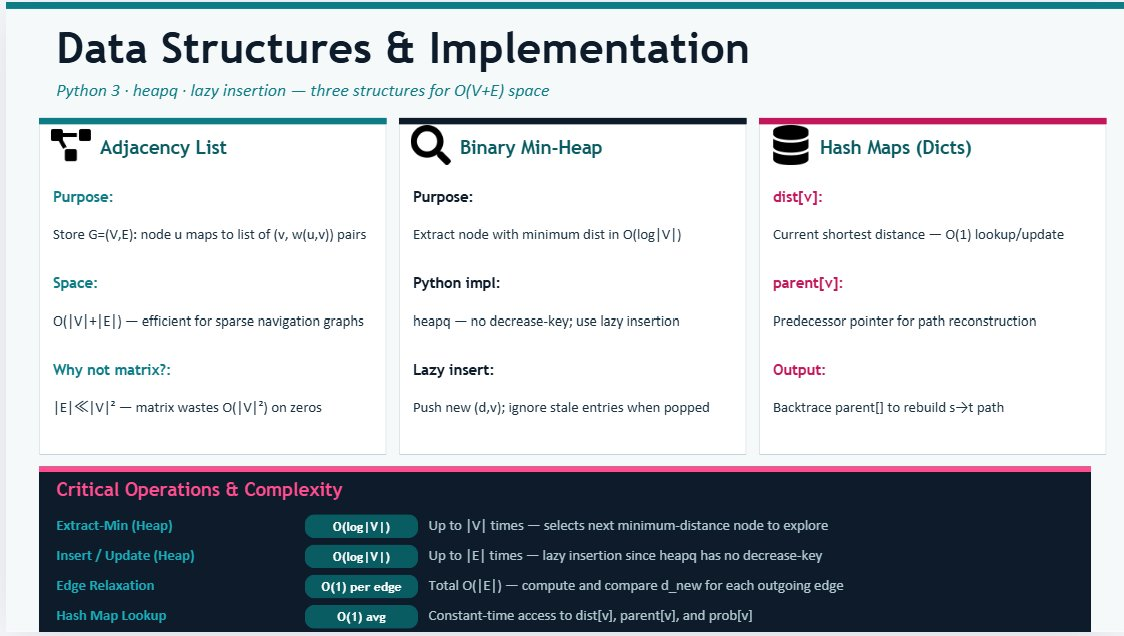
\includegraphics[width=0.95\textwidth]{data_structures.png}
\caption[$\tau$ sensitivity analysis: runtime speedup and optimality gap]{Anticipated $\tau$ sensitivity results. \textbf{Left:} Expected runtime speedup (Pruned / Baseline) at six threshold values $\tau \in \{10^{-6}, 10^{-4}, 10^{-3}, 0.01, 0.05, 0.2\}$, ranging from $1.00\times$ (baseline equivalent) to $2.40\times$. \textbf{Right:} Corresponding optimality gap $\Delta$ (\%), remaining near-zero for $\tau \leq 0.01$ and growing sharply beyond $\tau = 0.05$. Values are simulated projections to be validated experimentally. The trade-off confirms that the pruned algorithm can achieve significant efficiency gains with negligible accuracy loss at moderate threshold settings.}
\label{fig:tau_sensitivity}
\end{figure}

\section{Search Space Reduction}

\subsection{Nodes Explored and Edges Relaxed}

The pruned algorithm is expected to explore fewer nodes and relax fewer edges than the baseline across all tested configurations. The reduction is anticipated to become more pronounced as $\tau$ increases and as graph size grows, directly reducing the cumulative heap operation overhead.

\subsection{Max Priority Queue Size (MaxPQSize)}

The maximum frontier size during execution is expected to be consistently lower for the pruned algorithm, confirming that pruning controls heap growth. This metric will serve as empirical evidence that pruning improves practical runtime by limiting priority queue expansion beyond what is captured by edge relaxation counts alone.

\section{Optimality Gap Analysis}

For small values of $\tau$ (e.g., $\tau \leq 0.01$), the relative optimality gap:
\[
\Delta = \frac{|\Pi^*_{\text{baseline}} - \Pi^*_{\text{pruned}}|}{\Pi^*_{\text{baseline}}} \times 100\%
\]
is expected to remain within acceptable limits across all tested configurations. At higher values of $\tau$, the gap is anticipated to widen, reflecting the controllable trade-off between efficiency and optimality.

\section{Effect of Probability Distribution}

\subsection{Uniform Distribution}

Under uniformly distributed transition probabilities, pruning is expected to provide moderate search-space reduction. Because many paths will maintain similar cumulative probabilities, fewer partial paths are anticipated to fall below the pruning threshold, resulting in a smaller performance gap between baseline and pruned variants.

\subsection{Skewed (Power-Law) Distribution}

Under skewed probability distributions, a larger proportion of paths is expected to quickly accumulate low probabilities, triggering pruning more aggressively. This should produce greater runtime reductions and stronger frontier size control compared to the uniform case, suggesting that the pruned algorithm will be particularly effective in graphs with heterogeneous edge weights.

\section{Summary of Anticipated Outcomes}

A successful outcome is expected to demonstrate the following:
\begin{enumerate}
    \item The baseline Dijkstra algorithm will correctly compute globally optimal conversion paths in all tested instances, with empirical complexity consistent with $O(|E| \log |V|)$.
    \item The pruned Dijkstra algorithm will converge to the baseline solution as $\tau \to 0$, validating its correctness in the limit.
    \item For moderate $\tau$ values, the pruned algorithm will achieve measurable runtime improvements with small and controllable optimality gaps, presenting a clear efficiency--optimality trade-off curve.
    \item The performance advantage of pruning will be most pronounced in larger graphs and under skewed probability distributions.
    \item Empirical complexity results will be consistent with the theoretical analysis: $O(|E| \log |V|)$ for the baseline and $O(|E'| \log |V|)$ for the pruned variant, with $|E'| < |E|$ confirmed across experiments.
    \item The study will be reproducible, well-structured, and supported by systematic experimental evaluation across varying graph sizes and parameters.
\end{enumerate}

    \chapter{CONCLUSION}

\section{Summary}

This proposal presents an algorithmic workflow process for \textit{Customer Journey Path Optimization}, addressing the problem of identifying the most probable conversion path in large directed navigation graphs derived from user interaction data. The core formulation transforms the probabilistic path optimization problem into a shortest-path problem via the negative log-probability weight transformation~\citep{viterbi1967error,manning2008nlp}, enabling Dijkstra's algorithm~\citep{dijkstra1959} to be applied with correctness and complexity guarantees.

Two algorithms are proposed: a \textbf{baseline Dijkstra} that guarantees globally optimal solutions in $O(|E|\log|V|)$ time~\citep{cormen2009}, and a \textbf{probability-pruned Dijkstra} that extends the baseline with a threshold $\tau$ to discard low-probability partial paths during traversal. The pruned algorithm is expected to reduce execution time and peak memory usage by shrinking the effective search space and controlling priority queue growth, while converging exactly to the baseline as $\tau \to 0$.

\section{Expected Contributions}

The five contributions below are stated in terms of what is \emph{novel or distinctive} about this work relative to the gaps identified in the literature review (Chapter~2).

\begin{enumerate}

    \item \textbf{Unified probabilistic path optimization framework for customer journey graphs.}
    While existing work addresses shortest-path computation~\citep{dijkstra1959,cormen2009}, Markov chain modeling~\citep{norris1998markov}, and sequential pattern mining~\citep{pei2001prefixspan} as separate problems, this project integrates all three within a single algorithmic framework tailored to e-commerce conversion path analysis. This unification---combining the log-probability shortest-path formulation with threshold-controlled pruning---has not been studied in the context of navigation graph optimization.

    \item \textbf{Probability-threshold pruning as a principled approximation strategy.}
    Unlike heuristic approaches such as A*~\citep{hart1968astar} (which require an admissible heuristic over log-probability weights) or beam search (which provides no optimality guarantee), the proposed pruning strategy is parameter-controlled, deterministic, and formally guaranteed to converge to the optimal solution as $\tau \to 0$. This provides a more principled efficiency--optimality trade-off curve than existing approximation methods.

    \item \textbf{Empirical characterization of the time--memory--optimality trade-off.}
    Existing studies of large-scale graph systems~\citep{malewicz2010pregel,sahu2020scaling} focus on distributed scalability. This project provides a controlled, single-machine empirical analysis of how input size, edge density, and probability distribution jointly affect execution time, peak memory usage, and solution quality for both algorithms---a gap in the current experimental literature on navigation graph optimization.

    \item \textbf{Validated complexity analysis across three input scales.}
    The theoretical $O(|E|\log|V|)$ time and $O(|V|+|E|)$ space bounds~\citep{cormen2009} will be empirically validated across small, medium, and large graph instances, confirming that the complexity analysis holds in practice and identifying the threshold at which hardware constraints become binding.

    \item \textbf{Reproducible experimental framework for algorithm comparison on navigation graphs.}
    A fully specified simulation environment (Table~\ref{table:simenv}), standardized metrics including peak memory usage, and a synthetic graph generator with controlled structural parameters will be released as a reproducible benchmark, enabling future work to extend or compare against these results.

\end{enumerate}

\section{Anticipated Limitations}

\begin{itemize}
    \item \textbf{No formal approximation guarantee for $\tau > 0$:} The optimality gap is evaluated empirically; no worst-case bound is provided. Future work may derive a bound as a function of $\tau$ and the probability distribution~\citep{cormen2009}.
    \item \textbf{Limited benefit in dense or uniform graphs:} Pruning provides less search-space reduction when edge densities are high or transition probabilities are nearly uniform, as fewer paths fall below the threshold.
    \item \textbf{Hardware constraints:} Graphs approaching 50,000 nodes may reach RAM limits, potentially restricting the upper end of scalability experiments.
    \item \textbf{Single source--target pair:} Multi-query or all-pairs extensions are outside the current scope.
\end{itemize}

\section{Future Directions}

\begin{itemize}
    \item \textbf{Formal approximation bounds:} Characterizing the optimality gap as a function of $\tau$ and graph structure~\citep{cormen2009}.
    \item \textbf{Adaptive threshold selection:} Automatic $\tau$ tuning based on observed probability distribution statistics.
    \item \textbf{Bidirectional search:} Combining pruned Dijkstra with bidirectional expansion to further reduce the search frontier~\citep{cormen2009}.
    \item \textbf{Frequent journey pattern mining:} Integrating PrefixSpan~\citep{pei2001prefixspan} to identify common navigation paths alongside optimal path computation.
    \item \textbf{Dynamic graphs:} Extending the framework to handle time-varying transition probabilities~\citep{norris1998markov}.
\end{itemize}

\section{Concluding Remarks}

This project proposes a principled, efficient, and empirically evaluable approach to probabilistic path optimization in customer journey graphs. By combining the log-probability transformation~\citep{viterbi1967error}, Dijkstra's algorithm~\citep{dijkstra1959}, threshold-based pruning, and a fully specified experimental framework, the work addresses a genuine gap in the algorithmic literature on navigation graph analysis and contributes both theoretical clarity and practical benchmarking infrastructure for future research.

    \chapter{PROJECT PLAN}

\section{Project Timeline}

Figure~\ref{fig:timeline} presents the 10-week project timeline for the \textit{Probabilistic Path Optimization using Pruned Dijkstra} project. Tasks are organized in three overlapping phases: implementation (Weeks~1--4), testing and experimentation (Weeks~4--7), and analysis, writing, and presentation (Weeks~7--10). This phased structure ensures that correctness is validated before experimentation begins, and that experimental results directly inform the final report and presentation.

\begin{figure}[h!]
\centering
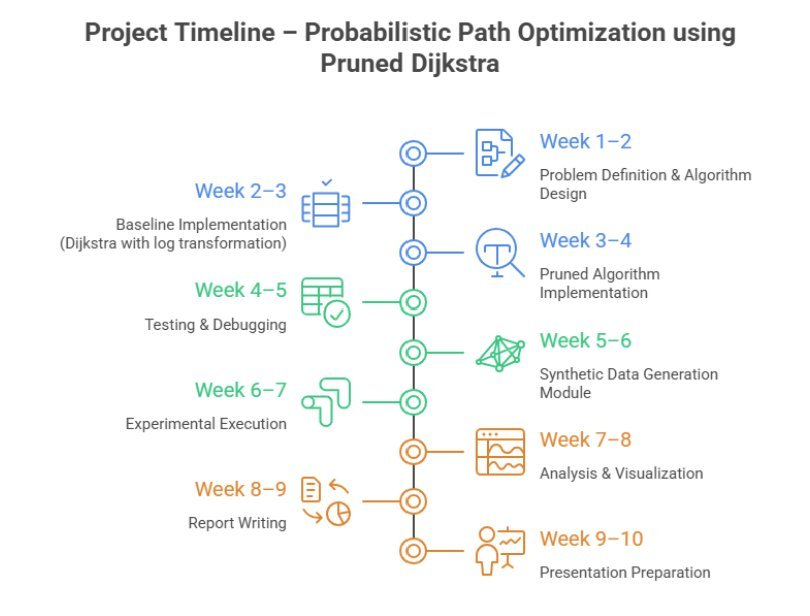
\includegraphics[width=0.85\textwidth]{timeline.png}
\caption[Project timeline]{Project timeline for \textit{Probabilistic Path Optimization using Pruned Dijkstra}. The timeline is structured across 10 weeks, alternating between left and right panels along a central spine. Blue entries correspond to the implementation phase (Weeks~1--4), green to the testing and experimentation phase (Weeks~4--7), and orange to the writing and presentation phase (Weeks~7--10). Each task overlaps with the subsequent one to allow iterative refinement.}
\label{fig:timeline}
\end{figure}

\section{Milestones}

The following milestones define the key delivery points of the project:

\begin{enumerate}
    \item \textbf{Core Implementation Completed:} End of Week~4\\
    Both the baseline Dijkstra algorithm and the probability-pruned Dijkstra algorithm will be fully implemented, tested on small hand-computed graphs, and validated for correctness against ground-truth optimal paths.

    \item \textbf{Experiments Completed:} End of Week~7\\
    All experimental runs across small, medium, and large graph configurations will be completed, with all metrics (execution time, peak memory, nodes explored, edges relaxed, optimality gap, MaxPQSize) recorded and verified.

    \item \textbf{Report Completed:} End of Week~9\\
    The full project report will be finalized, incorporating experimental results, visualizations, complexity validation, and the time--memory--optimality trade-off discussion.

    \item \textbf{Final Presentation Ready:} Week~10\\
    Presentation slides and a live demonstration of the implementation will be prepared for the final project presentation on 12~March~2026.
\end{enumerate}


    % ---- APA References ----
    \pagestyle{plain}
    \newpage
    \phantomsection
    \addcontentsline{toc}{chapter}{REFERENCES}
    \renewcommand{\bibsection}{%
      \chapter*{REFERENCES}%
    }
    \bibliographystyle{plainnat}
    \bibliography{references}

    % ---- Appendix ----
    \chapter*{APPENDIX A: SOURCE CODE AVAILABILITY}
\addcontentsline{toc}{chapter}{APPENDIX A: SOURCE CODE AVAILABILITY}

The implementation of the proposed \textit{Customer Journey Path Optimization} framework was developed in \textbf{Python 3}. The repository contains the baseline Dijkstra algorithm with log-transformed probabilities, the proposed probability-pruned Dijkstra variant, the synthetic dataset generation scripts, and the experimental evaluation scripts used in this study.

The complete source code is publicly available at:

\begin{center}
\textbf{\url{https://github.com/The-Two-Y-s/Customer-Journey-Path-Optimization}}
\end{center}

The repository includes:

\begin{itemize}
    \item Baseline Dijkstra implementation on log-transformed probability graphs
    \item Probability-Pruned Dijkstra implementation
    \item Synthetic graph generation module
    \item Experiment execution and benchmarking scripts
    \item Supporting utilities for evaluation and reproducibility
\end{itemize}

The implementation follows the same data structure choices described in this report, namely adjacency lists for sparse graph storage, a binary min-heap using Python's \texttt{heapq} for priority queue operations, and hash maps for distance tracking and path reconstruction.

This repository is provided to ensure transparency, reproducibility, and ease of further extension of the proposed algorithms.

\end{document}